\chapter{能谱成像与阿秒传播}
\label{chap:pinem-measurements}

前章得到的是给定电子轨迹的复振幅 $c_n(\vb R)$。束流并不只有一条轨迹：入射位置和到达时刻都有分布，探测器又将真实边带映射为有限分辨率的计数。因此实际图像需要从单电子振幅出发，先决定哪些相干性被保留，再对未分辨的实验变量求平均。

本章直接完成一次从假定近场到实际能谱的前向计算。在没有指定结构材料以前，近场包络被明确视为教学模型；等到后面需要确定其绝对幅度、相位与材料共振时，再求解 Maxwell 方程和球形边界问题。这一区分使眼前的实验预测可复核，又不会把经验近场误说成电磁边值问题的精确解。

电子的能谱只保留能量阶数，而一个带角相位的近场还会把信息编码到出射电子的轨道角动量中。即使理想能量谱完全相同，两种角相位纹理也可能在高阶能量--OAM 联合谱中区分；反过来，增加一个相干参考可以改变原来的不可辨识性。本章先给出能量与束流的读出链，相关的角相位和参考设计在后面的合成维度与测量章节给出完整计算。


\section{束流成像}
单条轨迹的相干边带由贝塞尔展开确定，但实验中的电子并非全部沿同一条轨迹经过结构。要把局域边带概率转成可测强度，必须知道探针经过各个横向位置的概率，以及仪器如何把真实能量变成计数。设横向入射概率密度为 $w(\vb R)$，它满足 $w\geq0$ 和 $\int w(\vb R)\,\dd^2R=1$。对单个撞击位置，能量边带概率是 $J_n^2(2|\beta(\vb R)|)$；不读取撞击位置时，实测的理想通道概率是
\begin{equation}
\overline P_n=\int\!w(\vb R)J_n^2(2|\beta(\vb R)|)\,\dd^2R.
\label{eq:beam-averaged-pinem-probability}
\end{equation}
不同轨迹在这里以概率而非复振幅相加，因为其横向路径信息已被平均。这不是说单条轨迹上的相干性已经消失；当实验能够固定或相干选择横向末态时，必须恢复相应振幅层级的描述。

若入射能量与探测器的总响应为单位面积的 $G_{\sigma_E}$，最终能谱才是
\begin{equation}
I(E)=\sum_{n\in\ZZ}\overline P_n\,
G_{\sigma_E}(E-E_0-n\hbar\omega).
\label{eq:averaged-observed-pinem-spectrum}
\end{equation}
两次操作的顺序不能随意互换：对非线性的 $J_n^2$ 先作 $\beta$ 平均通常给出错误结果；但对已经求出的概率作积分与线性卷积可以交换次序。对于能量选择成像，测量器将某些 $n$ 通道相加成一个像素强度；对于全谱分析，则保留 $E$ 依赖。这个从近场轨迹到计数的公式，才是连接实际样品与实验图像的前向模型。

这些公式可以直接对照最早的 PINEM 实验。它们先回答电子如何从局域场交换离散能量，再回答能量选择后的信号为什么形成空间和时间上的近场图像。

Barwick 等在 2009 年首先把离散能量交换、时间门控和近场成像放在同一实验链条中。\textsuperscript{\hyperref[ch01-ref1]{[1]}}
论文首先比较电子与激光错开和时间重合时的能谱。只有在纳米结构处同时满足空间和时间重合，200 keV 电子才出现以约 2.4 eV 为间隔的能量增益和损失峰；最大重合时可见到多个高阶量子。这个观察先解决了最基本的问题：自由空间中受能量—动量守恒禁止的单光子交换，在纳米结构产生的局域场中可以发生。

第二步不是继续分析峰形，而是只选择获得能量的电子成像。这样图像中的亮度直接来自发生了光子交换的电子。论文由此测得近场只分布在纳米结构附近，真空侧的特征延伸尺度约为 50 nm；再扫描电子—光延迟，得到约数百飞秒的瞬态门。最后改变入射光偏振，证明图像对纳米结构几何与局域场方向敏感。

因此这篇论文的逻辑是“离散能量交换 → 能量筛选 → 空间成像 → 时间扫描 → 偏振扫描”。它主要给出实验事实，并没有从贝塞尔函数出发建立强场理论；这里直接把论文报告的能量间隔、时间宽度和空间尺度作为实验尺度证据，并与前面的统一模型对应起来；这些尺度不是原始计数数据的数字化。


随后，García de Abajo 的强场理论把这些边带写成相干多路径振幅，而不是独立泊松事件。\textsuperscript{\hyperref[ch01-ref2]{[2]}}
Barwick 的实验已经证明多光子交换存在，但还不能解释不同边带为什么随光强出现明显的非泊松振荡。论文从含时散射问题出发，把电子波函数按散射阶数 $N$ 和净交换光子数 $L$ 展开。不同 $N$ 可以到达同一个最终 $L$，所以这些路径必须先相干相加。

有限脉冲的一般结果写成论文式 (10)：$P_L$ 同时含有不同散射阶数的交叉项，并显式依赖 $\tau/\Delta_p$ 与 $\Delta_e/\Delta_p$。当电子脉冲远短于光脉冲时，式 (10) 化成论文式 (11)；这时相干路径干涉最清楚。随着光强增加，低阶通道可以先增强再被抽空，概率转移到更高阶，这就是论文图 2 的主要结论。

电子脉冲变长时，不同相互作用时刻对应的振幅被平均，路径相消的细结构被洗掉；改变延迟则主要降低电子看到的有效场强。因此数值模型必须明确区分“点电子/连续波极限”和“有限脉冲平均”，不能把后者误写成一个单纯的贝塞尔公式。


Park 等进一步把近场傅里叶匹配、贝塞尔边带和有限脉冲平均连成一条前向模型。\textsuperscript{\hyperref[ch01-ref3]{[3]}}
这篇长文先处理能量—动量匹配。对给定光子频率 $\omega$，电子要沿轨迹连续吸收能量，需要纵向空间频率接近 $k_z=\omega/v_e$。自由空间光只有 $k_z\le\omega/c$，而 $v_e<c$，所以单个传播光子不能满足条件；纳米结构的空间局域性提供了额外的大波矢分量。

接着论文先解纳米结构的电磁散射。小颗粒用瑞利极限说明场的尺寸、材料和偏振标度，更一般的尺寸用 Mie 展开。得到 $E_z$ 后，真正进入电子动力学的不是峰值场，而是论文定义的纵向傅里叶分量 $\widetilde F_z(\omega/v_e)=\int \dd z\,E_z(z)\ee^{-\ii\omega z/v_e}$。

最后才解含时薛定谔方程。Jacobi--Anger 展开把相位调制写成离散能量波包，连续波极限给出 $P_n=J_n^2(|e\widetilde F_z/(\hbar\omega)|)$；有限电子和光脉冲则要再对包络积分。论文随后逐项与空间分布、偏振、能谱、延迟和光通量实验比较。这个顺序非常重要：电磁场 → 轨迹傅里叶选择 → 电子相位 → 边带概率 → 实验平均。


在 200 keV 区域，相对论运动学必须进入模型；Park 与 Zewail 说明了窄带正能波包下 Dirac 与常用包络描述怎样兼容。\textsuperscript{\hyperref[ch01-ref4]{[4]}}
论文提出的问题非常具体：PINEM 实验使用 200 keV 电子，非相对论速度会给出约 $0.885c$，而正确相对论速度约为 $0.7c$。既然相位匹配直接含 $\omega/v$，速度用错会明显改变结果。

作者分别从薛定谔和 Dirac 方程建立一阶相互作用，并证明：只要在薛定谔包络方程中使用相对论修正后的 $v$、$p$ 和对应载波能量，一阶 PINEM 转移概率与 Dirac 结果等价。补充材料进一步说明，200 keV 附近几个 eV 的能量展开只让正能 Dirac 旋量系数发生极小变化，因此可以把旋量近似固定，把主要动力学留在标量包络中。

这篇论文不是说“相对论可以忽略”，而是说相对论主要通过正确的运动学参数进入一阶 PINEM 包络。这个结论的适用范围是论文所讨论的一阶、窄能宽、正能电子波包。


Feist 等随后直接观测到多能级相干人口振荡，使“能量晶格上的相干传播”成为实验上可检验的语言。\textsuperscript{\hyperref[ch01-ref5]{[5]}}
论文把相互作用写成 $S=\exp(g^*a-ga^\dagger)$。这里的 $a$ 与 $a^\dagger$ 不是谐振子产生湮灭算符，而是把自由电子能量平移一个光子量子的通道算符；相邻能量阶之间的耦合近似相同，因此所有边带由同一个复数 $g$ 控制。

直接结果是 $P_N=|J_N(2|g|)|^2$。实验随入射场强扫描时，零损峰和各阶边带都出现消失与复现；作者用一个线性标定 $2|g|=98F_{inc}$（$F_{inc}$ 以 V nm$^{-1}$ 计）同时拟合多个阶数。这一点比“出现很多边带”更强：不同最终能量通道共享同一相干演化参数。

相互作用结束后，电子已经获得周期谱相位。自由传播给不同能量分量不同传播相位，于是能量调制转成时间密度调制。论文数值结果在约 1.8 mm 传播后得到约 80 as 的脉冲列。


前面的结果依赖两类近似。第一类近似作用在电磁场模型上，例如把小颗粒当成偶极子；第二类近似作用在电子传播上，例如把 $p(E+n\hbar\omega)$ 对能量作线性展开。两类近似的控制参数不同，所以必须分别检查：尺寸增大时看多极展开是否收敛，交换阶数增大或电子能量降低时看反冲修正是否仍小。

\begin{figure}[!htbp]
\centering
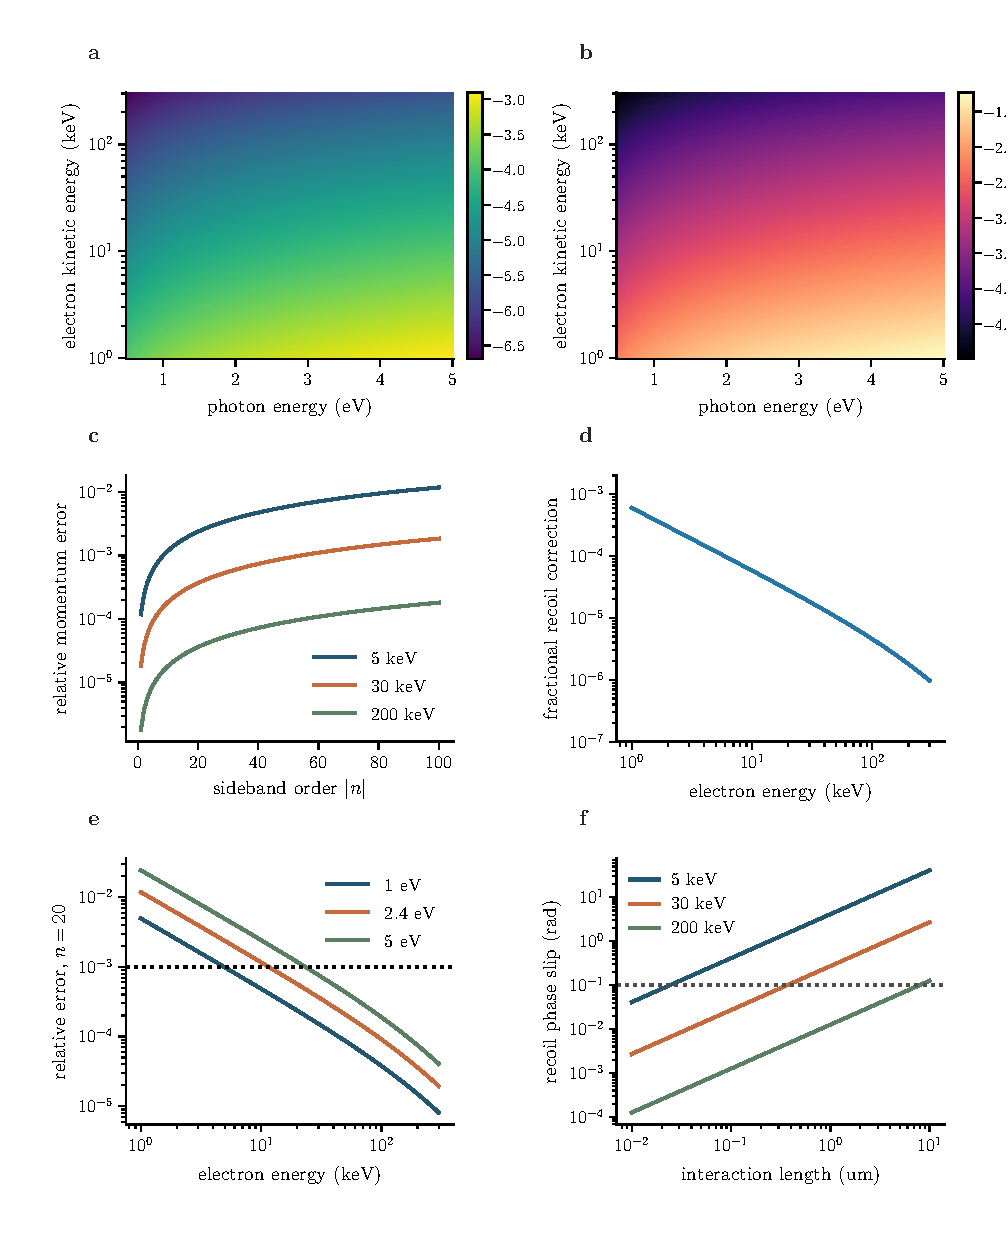
\includegraphics[width=0.96\linewidth,height=0.70\textheight,keepaspectratio]{recoil_approximation_breakdown.pdf}
\caption{\textbf{无反冲近似的误差与相位积累。} (a,b) 单光子与五十光子交换时的相对动量误差；(c) 误差对交换阶数的依赖；(d) 在 $2.4\,\mathrm{eV}$ 下展示单光子相对修正 $|q^{\rm ex}/q^{(0)}-1|$，避免重合的动量曲线；(e) 多光子相对误差与 $10^{-3}$ 阈值；(f) 长度 $L$ 上累积的反冲相位误差，虚线为 $0.1$ 弧度。图中误差均直接由相对论动量--动能关系计算。}
\label{fig:ch01-novel-extensions--33-recoil-approximation-breakdown}
\end{figure}

采用相对论动量—动能关系，并直接比较有限交换阶数下的动量差：
\[\begin{aligned}
p(K)&=\frac{1}{c}\sqrt{K(K+2m_ec^2)}, & q_n^{\rm ex}&=\frac{p(K+n\hbar\omega)-p(K)}{\hbar},\\
q_n^{(0)}&=\frac{n\omega}{v(K)}, & \epsilon_q&=\frac{|q_n^{\rm ex}-q_n^{(0)}|}{|q_n^{\rm ex}|},\\
\delta\varphi&=L|q_n^{\rm ex}-q_n^{(0)}|.
\end{aligned}\]
取 $K\in[1,300]\,\mathrm{keV}$（150 个对数采样点），$\hbar\omega\in[0.5,5]\,\mathrm{eV}$（150 点）；比较 $n=1,20,50$ 和 $1\le |n|\le100$，以及 $K=5,30,200\,\mathrm{keV}$、$\hbar\omega=2.4\,\mathrm{eV}$；第六面板固定 $|n|=20$，改变 $L\in[0.01,10]\,\mathrm{\mu m}$，参考相位误差阈值 $0.1$ rad。这是运动学近似误差而非完整多通道散射误差。


取最简单的有限作用区。电子沿 $z$ 方向匀速通过近场，作用区为 $-L/2\le z\le L/2$，纵向电场近似为 $E_z(z)=E_0\ee^{\ii k_z z}$。把它代入复耦合的定义，得到

\begin{equation*}
\beta=\frac{eE_0}{2\hbar\omega}\int_{-L/2}^{L/2}\ee^{\ii(k_z-\omega/v)z}\,\dd z.
\end{equation*}

记波矢失配为 $\Delta k=k_z-\omega/v$。积分只含一个指数函数，因此可以直接算出

\begin{equation}
\beta=\frac{eE_0L}{2\hbar\omega}\,\operatorname{sinc}\!\left(\frac{\Delta kL}{2}\right),\qquad \operatorname{sinc}x\equiv\frac{\sin x}{x}.
\label{eq:ch01-6}
\end{equation}

当 $\Delta k=0$ 时，各位置贡献的相位相同，$|\beta|$ 与作用长度 $L$ 成正比。失配增大后，作用区前后两端的贡献开始相消。第一个零点满足 $|\Delta k|L/2=\pi$，所以接受带宽的自然尺度为 $|\Delta k|\sim2\pi/L$。作用区越长，峰值耦合越强，但允许的波矢失配越小。

最后把\cref{eq:ch01-6} 代入 $P_n=J_n^2(2|\beta|)$，即可得到有限长度作用区的能谱。计算时先由材料响应与几何确定 $E_z$，再进行轨迹积分求 $\beta$，最后结合贝塞尔边带分布及仪器响应预测可测谱线。


单个参数点只能说明“在这里会看到什么”，不能说明模型在哪些区域可靠。把 $|\beta|$、失配量 $\Delta kL$ 和分辨率 $\sigma_E/\hbar\omega$ 连续扫描，可以直接划出弱耦合、多光子、失配和不可分辨区域。真正有用的是这些区域之间的边界。


不过将复杂电磁场压缩为一个复数并非没有代价。下面从偏折、反冲和作用区长度出发，逐一检查经典轨迹近似何时可靠。
主模型建立以后，还要检查实验平均和噪声是否改变结论。有限脉冲会把不同瞬时 $\beta$ 的概率加权平均；空间不均匀会把不同撞击参数对应的谱混合；相位噪声则首先压低密度矩阵的非对角元。它们改变的物理量不同，所以不能用同一个“有效耦合减小”来概括。


\par\medskip
前面的实验模型把每次电子相互作用视为固定耦合。实际光场只在有限时间内存在，电子到达时刻的变化会改变轨迹上的有效相位。由连续波的边带公式推广到有限脉冲时，必须先计算每次到达对应的复振幅，再决定何种探测条件允许作概率平均。
\par\medskip


\section{有限脉冲}
固定一条纵向特征线，定义
\begin{equation}
\zeta\equiv z-v_0t,\qquad z(t')=\zeta+v_0t'.
\label{eq:moving-coordinate}
\end{equation}
在时间规范 $\phi=0$ 下，式~\cref{eq:eikonal-phase-general} 直接给出
\begin{align}
\frac{g(\zeta,t)}{g(\zeta,t_0)}
&=\exp\left[
\frac{\ii q_{\rm e}v_0}{\hbar}
\int_{t_0}^{t} A_z(\zeta+v_0t',t')\,\dd t'
\right].
\label{eq:g-integral}
\end{align}
这里没有重新建立运动方程：只是把前文的通用特征线写成一维随动坐标。下面所有脉冲修正都从这个已经闭合的母式出发。


对准单色脉冲，必须区分“频域 phasor”与“含慢包络的正频时域场”。把前文的空间 phasor 记作 $E_{\omega,z}(z)$，并定义正频部分
\begin{equation}
 E_z^{(+)}(z,t)
 \equiv E_{\omega,z}(z)\,
 a_{\rm L}(t-\tau)\,
 \ee^{-\ii\omega t},
 \qquad
 a_{\rm L}(t-\tau)
 =\exp\left[-\frac{(t-\tau)^2}{4\sigma_{\mathrm L}^2}\right].
 \label{eq:complex-field}
\end{equation}
真实电场仍是 $E_z=\operatorname{Re}E_z^{(+)}$。准单色条件不是一句“脉冲很长”，而是慢包络的相对变化率小于载频：
\begin{equation}
 {
 \epsilon_{\rm SVEA}(t)
 \equiv
 \frac{|\partial_t a_{\rm L}(t-\tau)|}
 {\omega |a_{\rm L}(t-\tau)|}
 =
 \frac{|t-\tau|}{2\omega\sigma_{\rm L}^2}
 \ll1}
 \label{eq:SVEA-field-condition}
\end{equation}
在脉冲主要支撑区 $|t-\tau|\lesssim\sigma_{\rm L}$ 内，一个简单充分条件就是
\begin{equation}
 {\omega\sigma_{\rm L}\gg1.}
 \label{eq:quasimonochromatic-condition}
\end{equation}

但式~\cref{eq:complex-field} 还隐含了另一件与“载频远大于带宽”不同的事情：整个脉冲带宽内，纳米结构的空间场型也必须近似不变，否则不能把完整频谱写成一个固定的 $E_{\omega,z}(z)$ 乘同一个时间包络。记脉冲特征带宽为 $\Delta\omega_{\rm L}\sim\sigma_{\rm L}^{-1}$，并用 $\|\cdot\|_{\rm int}$ 表示在电子实际采样区域上的一致场范数，则一个局部充分条件是
\begin{equation}
{
\epsilon_{\rm mode}
\equiv
\Delta\omega_{\rm L}
\frac{\|\partial_\omega E_{\omega,z}\|_{\rm int}}
{\|E_{\omega,z}\|_{\rm int}}
\ll1.}
\label{eq:pulse-spatial-mode-freeze}
\end{equation}
式~\cref{eq:quasimonochromatic-condition} 控制时间载波与慢包络的分离，式~\cref{eq:pulse-spatial-mode-freeze} 控制材料色散和几何共振在脉冲带宽内是否可以冻结。靠近窄线宽 Mie 或材料共振时，前者可能成立而后者失效；此时必须保留 $\vb E_{\Omega}(\vb r)$ 的频率依赖并对光谱逐频积分，而不能只给单频 $\beta$ 乘一个时间 Gaussian。

为了把一阶输运式~\cref{eq:g-integral} 写成电场形式，这里选择 $\phi=0$ 的时间规范；这是计算上的规范选择，不是新的物理近似。相应正频矢势写成
\begin{equation}
 A_z^{(+)}(z,t)
 =\mathcal A_z(z,t)\ee^{-\ii\omega t}.
\end{equation}
由 $E_z^{(+)}=-\partial_tA_z^{(+)}$，
\begin{align}
E_z^{(+)}
&=-\left[(\partial_t\mathcal A_z)-\ii\omega\mathcal A_z\right]
 \ee^{-\ii\omega t}\\
&=\left[\ii\omega\mathcal A_z-\partial_t\mathcal A_z\right]
 \ee^{-\ii\omega t}.
\end{align}
在式~\cref{eq:SVEA-field-condition} 控制下，$\partial_t\mathcal A_z$ 相对 $\omega\mathcal A_z$ 是一阶小量。为了不把无量纲误差直接加到有量纲矢势上，显式定义余项 $\delta A_z^{(+)}$：
\begin{equation}
 A_z^{(+)}(z,t)
 =\frac{E_z^{(+)}(z,t)}{\ii\omega}
 +\delta A_z^{(+)}(z,t),
 \qquad
 \frac{|\delta A_z^{(+)}|}{|E_z^{(+)}|/\omega}
 =O(\epsilon_{\rm SVEA}).
 \label{eq:A-from-E-positive-frequency}
\end{equation}
取实部得到真正代入电子相位积分的实矢势
\begin{equation}
 A_z(z,t)
 =\frac{1}{\omega}\operatorname{Im}E_z^{(+)}(z,t)
 +\delta A_z(z,t),
 \qquad
 |\delta A_z|=O\!\left(\epsilon_{\rm SVEA}\frac{|E_z^{(+)}|}{\omega}\right).
 \label{eq:A-from-E}
\end{equation}
因此 SVEA 的误差不是一个孤立的无量纲加数，而是相对于主矢势 $|E^{(+)}|/\omega$ 的相对误差。

将式~\cref{eq:complex-field} 与 \cref{eq:A-from-E} 逐项代入式~\cref{eq:g-integral}：
\begin{align}
 \frac{g(z',t)}{g(z',t_0)}
 =\exp\Bigg\{\ii\frac{q_{\rm e}v_0}{\hbar\omega}
 \int_{t_0}^{t}\dd t'\,
 \operatorname{Im}\Bigg[
 &E_{\omega,z}(z'+v_0t')\ee^{-\ii\omega t'}\notag\\
 &\times\exp\left(-\frac{(t'-\tau)^2}{4\sigma_{\mathrm L}^2}\right)
 \Bigg]\Bigg\}.
 \label{eq:time-integral-E}
\end{align}
令
\begin{equation}
 z''=z'+v_0t',
 \qquad
 t'=\frac{z''-z'}{v_0},
 \qquad
 \dd t'=\frac{\dd z''}{v_0}.
 \label{eq:zpp-change}
\end{equation}
则
\begin{align}
 \ee^{-\ii\omega t'}
 &=\exp\left[-\ii\frac{\omega}{v_0}(z''-z')\right]\\
 &=\ee^{+\ii(\omega/v_0)z'}
 \ee^{-\ii(\omega/v_0)z''},
 \label{eq:phase-change}
\end{align}
而脉冲包络变成
\begin{equation}
 \exp\left[-\frac{(z''-z'-v_0\tau)^2}{4v_0^2\sigma_{\mathrm L}^2}\right].
 \label{eq:pulse-in-zpp}
\end{equation}
到这一步还没有假定光脉冲在电子穿越近场期间保持不变。先把有限积分区间扩展到整条轨迹。若初、末时刻选在相互作用完全结束之后，使截去的尾部满足
\begin{equation}
 {
 \int_{-\infty}^{t_0}\!|A_z(z'+v_0t',t')|\,\dd t'
 +\int_t^{+\infty}\!|A_z(z'+v_0t',t')|\,\dd t'
 \ll
 \int_{t_0}^{t}\!|A_z(z'+v_0t',t')|\,\dd t',}
 \label{eq:infinite-limit-condition}
\end{equation}
就可以令 $t_0\to-\infty$、$t\to+\infty$。把式~\cref{eq:phase-change} 和脉冲包络~\cref{eq:pulse-in-zpp} 代回式~\cref{eq:time-integral-E}。为了同时记录 $A$--$E$ 转换带来的误差，定义相互作用区上的最大慢变参数与主相位尺度
\begin{align}
\epsilon_{\rm SVEA}^{\max}
&\equiv \sup_{t'\in I_{\rm int}}\epsilon_{\rm SVEA}(t'),\\
\Phi_*
&\equiv
\frac{|q_{\rm e}|v_0}{\hbar\omega}
\int_{I_{\rm int}}\!\dd t'\,
|E_z^{(+)}(z'+v_0t',t')|,
\label{eq:pulse-phase-error-scale}
\end{align}
其中 $I_{\rm int}$ 是场与电子显著重叠的时间区间。由式~\cref{eq:A-from-E}，遗漏矢势在指数中造成的无量纲相位误差至多为 $O(\epsilon_{\rm SVEA}^{\max}\Phi_*)$。因此
\begin{align}
\frac{g(z',+\infty)}{g(z',-\infty)}
=\exp\Bigg\{
\ii\frac{q_{\rm e}}{\hbar\omega}
\operatorname{Im}\Bigg[
\ee^{\ii\kappa z'}
\int_{-\infty}^{+\infty}\dd z''\,
&E_{\omega,z}(z'')\ee^{-\ii\kappa z''}\\
&\times
 a_{\rm L}\!\left(\frac{z''-z'}{v_0}-\tau\right)
\Bigg]
+O(\epsilon_{\rm SVEA}^{\max}\Phi_*)
\Bigg\}.
\label{eq:pulse-phase-before-freeze}
\end{align}
因此在只使用 SVEA、尚未使用“穿越时间短”近似时，自然出现的是一个\emph{脉冲加权的轨迹 Fourier 投影}
\begin{equation}
{
\mathcal F_{\parallel}^{({\rm p})}(z',\tau)
\equiv
\int_{-\infty}^{+\infty}\dd z''\,
E_{\omega,z}(z'')\,
 a_{\rm L}\!\left(\frac{z''-z'}{v_0}-\tau\right)
\ee^{-\ii\kappa z''}.}
\label{eq:pulse-weighted-F}
\end{equation}
对应的慢变复耦合定义为
\begin{equation}
{
\beta_{\rm p}(z',\tau)
\equiv-\frac{q_{\rm e}}{2\hbar\omega}
\mathcal F_{\parallel}^{({\rm p})}(z',\tau).}
\label{eq:pulse-weighted-beta}
\end{equation}
于是式~\cref{eq:pulse-phase-before-freeze} 可写成与连续波完全同构的形式
\begin{equation}
{
\frac{g(z',+\infty)}{g(z',-\infty)}
=
\exp\left[
-\beta_{\rm p}(z',\tau)\ee^{\ii\kappa z'}
+\beta_{\rm p}^*(z',\tau)\ee^{-\ii\kappa z'}
+O(\epsilon_{\rm SVEA}^{\max}\Phi_*)
\right].}
\label{eq:pulse-phase-beta-exact-svea}
\end{equation}
这条式子非常重要：若脉冲持续时间与电子穿越近场的时间可比，并不需要重新建立电子动力学，只需要保留式~\cref{eq:pulse-weighted-F} 中空间场与时间包络的卷积；后面的“局域 $\beta$”只是它的进一步特殊极限。

现在才考察何时可以把光包络从近场积分中提出。设近场只在 $|z''|\lesssim L_{\rm nf}$ 内显著。对 Gaussian 包络，指数为
\begin{equation}
-\frac{(z''-z'-v_0\tau)^2}{4v_0^2\sigma_{\rm L}^2}.
\end{equation}
与 $z''=0$ 处相比，其变化量为
\begin{align}
 \left|
 \frac{(z''-z'-v_0\tau)^2-(-z'-v_0\tau)^2}
 {4v_0^2\sigma_{\rm L}^2}
 \right|
 &=\left|
 \frac{z''^2-2z''(z'+v_0\tau)}
 {4v_0^2\sigma_{\rm L}^2}
 \right|\ll1.
 \label{eq:pulse-freeze-exact}
\end{align}
对所有 $|z''|\le L_{\rm nf}$，一个充分条件是
\begin{equation}
 {
 \frac{L_{\rm nf}^2}{4v_0^2\sigma_{\rm L}^2}
 +\frac{L_{\rm nf}|z'+v_0\tau|}{2v_0^2\sigma_{\rm L}^2}
 \ll1.}
 \label{eq:pulse-freeze-condition}
\end{equation}
在电子与光脉冲主要重叠的区域 $|z'+v_0\tau|\lesssim v_0\sigma_{\rm L}$ 内，更直观的充分条件是
\begin{equation}
 {
 T_{\rm tr}\equiv\frac{L_{\rm nf}}{v_0}\ll\sigma_{\rm L}.}
 \label{eq:transit-condition}
\end{equation}
此时
\begin{equation}
 a_{\rm L}\!\left(\frac{z''-z'}{v_0}-\tau\right)
\simeq
 a_{\rm L}\!\left(-\frac{z'}{v_0}-\tau\right)
=
\exp\left[-\frac{(z'+v_0\tau)^2}{4v_0^2\sigma_{\rm L}^2}\right].
\label{eq:pulse-freeze}
\end{equation}
所以脉冲加权投影才进一步因式分解为
\begin{align}
\mathcal F_{\parallel}^{({\rm p})}(z',\tau)
&\simeq
\exp\left[-\frac{(z'+v_0\tau)^2}{4v_0^2\sigma_{\rm L}^2}\right]
\int_{-\infty}^{+\infty}
E_{\omega,z}(z'')\ee^{-\ii\kappa z''}\dd z''\\
&=
\exp\left[-\frac{(z'+v_0\tau)^2}{4v_0^2\sigma_{\rm L}^2}\right]
\mathcal F_{\parallel}(\kappa),
\label{eq:pulse-F-factorization}
\end{align}
其中
\begin{equation}
 \kappa\equiv\frac{\omega}{v_0},
 \qquad
 \mathcal F_{\parallel}(\kappa)
 \equiv\int_{-\infty}^{+\infty}
 E_{\omega,z}(z'')\ee^{-\ii\kappa z''}\,\dd z''.
 \label{eq:Fdef}
\end{equation}
因此
\begin{equation}
\beta_{\rm p}(z',\tau)
\simeq
\beta\,
\exp\left[-\frac{(z'+v_0\tau)^2}{4v_0^2\sigma_{\rm L}^2}\right],
\qquad
\beta=-\frac{q_{\rm e}}{2\hbar\omega}\mathcal F_{\parallel}.
\label{eq:pulse-beta-factorization}
\end{equation}
代回式~\cref{eq:pulse-phase-beta-exact-svea}，得到常用的局域相位形式
\begin{equation}
 {
 \frac{g(z',+\infty)}{g(z',-\infty)}
 =\exp\left\{
 \ii\frac{q_{\rm e}}{\hbar\omega}
 \operatorname{Im}\left[
 \ee^{\ii\kappa z'}\mathcal F_{\parallel}(\kappa)
 \right]
 \exp\left[-\frac{(z'+v_0\tau)^2}{4v_0^2\sigma_{\rm L}^2}\right]
 \right\}.}
 \label{eq:phase-final}
\end{equation}
因此有限脉冲理论有清楚的两层结构：式~\cref{eq:pulse-weighted-F} 是 SVEA 下仍保留穿越时间效应的一般结果；只有在 $T_{\rm tr}/\sigma_{\rm L}\ll1$ 后，才退化为“连续波 $\beta$ 乘局域光包络”的常用模型。


从本节开始额外采用式~\cref{eq:transit-condition} 的短穿越条件，因此可以使用已经因式分解的局域耦合~\cref{eq:pulse-beta-factorization}。若该条件不成立，应停留在脉冲加权耦合~\cref{eq:pulse-weighted-beta}，而不能把连续波 $\beta$ 简单乘上到达时刻的光包络。有限脉冲概率仍不需要重新使用正、负能基底。记
\[
g_0(\zeta)\equiv g(\zeta,-\infty).
\]
耦合强度使用\cref{eq:beta-standard} 定义的 $\beta$，并记 Bessel 自变量 $\eta=2|\beta|$：
\[
\eta=2|\beta|=\frac{e|\mathcal F_{\parallel}|}{\hbar\omega}.
\]
对于高斯光脉冲，局域耦合参数为
\begin{equation}
\eta_{\rm loc}(\zeta,\tau)
=
\eta
\exp\left[
-\frac{(\zeta+v_0\tau)^2}
{4v_0^2\sigma_{\mathrm L}^2}
\right].
\label{eq:eta-local}
\end{equation}
电子电荷的负号只影响边带复振幅的相位约定；概率只依赖 $|\eta_{\rm loc}|$。

先说明有限脉冲概率为什么是“局域 Bessel 权重的积分”，而不是把这一形式当作经验平均。式~\cref{eq:phase-final} 在固定 $\zeta=z'$ 处仍然只是一个正弦相位。把高斯实包络吸收到
\begin{equation}
\beta_{\rm loc}(\zeta,\tau)
\equiv
\beta\exp\!\left[-\frac{(\zeta+v_0\tau)^2}{4v_0^2\sigma_{\rm L}^2}\right],
\qquad
2|\beta_{\rm loc}|=\eta_{\rm loc},
\label{eq:beta-local-def}
\end{equation}
则正文已经固定的能量增益约定~\cref{eq:sideband-amplitude-gain-convention} 可以逐点使用：
\begin{align}
g(\zeta,+\infty)
&=\sum_{n=-\infty}^{+\infty}
\ee^{+\ii n\kappa\zeta}\,g_n(\zeta),
\label{eq:pulse-sideband-decomposition}\\
g_n(\zeta)
&=g_0(\zeta)
J_n\!\left(2|\beta_{\rm loc}(\zeta,\tau)|\right)
\ee^{\ii n\arg[-\beta_{\rm loc}(\zeta,\tau)]}.
\label{eq:pulse-local-sideband-amplitude}
\end{align}
快速因子 $\ee^{+\ii n\kappa\zeta}$ 把第 $n$ 个分量的中心波数移到
$k_0+n\kappa$；$g_n(\zeta)$ 则是围绕该中心的慢包络。高斯光包络为实正数时，$\arg\beta_{\rm loc}=\arg\beta$，所以所有空间依赖都只进入 Bessel 自变量。
若相邻边带的中心波数间隔
\begin{equation}
\Delta k_{\rm sb}=\frac{\omega}{v_0}
\end{equation}
远大于单个边带自身的谱宽 $\Delta k_{\rm env}$，即
\begin{equation}
{\Delta k_{\rm env}\ll \omega/v_0,}
\label{eq:sideband-orthogonality-general}
\end{equation}
则不同 $n$ 的动量支撑近似互不重叠。第 $n$ 个谱峰的总概率可以单独积分。为避免把“中心波数平移”藏在记号里，先对第 $n$ 个完整分量
$h_n(\zeta)\equiv\ee^{\ii n\kappa\zeta}g_n(\zeta)$ 作 Fourier 变换。若
\begin{equation}
\widetilde g_n(k)=\frac{1}{\sqrt{2\pi}}
\int g_n(\zeta)\ee^{-\ii k\zeta}\dd\zeta,
\end{equation}
则逐项代入得
\begin{align}
\widetilde h_n(k)
&=\frac{1}{\sqrt{2\pi}}
\int g_n(\zeta)\ee^{-\ii(k-n\kappa)\zeta}\dd\zeta\\
&=\widetilde g_n(k-n\kappa).
\label{eq:finite-pulse-fourier-shift}
\end{align}
因此完整谱峰只是慢包络谱向 $k=n\kappa$ 的平移，积分范数不变。Parseval 定理给出
\begin{align}
P_n
&=\int_{-\infty}^{+\infty}|\widetilde g_n(k)|^2\dd k\\
&=\int_{-\infty}^{+\infty}|g_n(\zeta)|^2\dd\zeta\\
&=\int_{-\infty}^{+\infty}|g_0(\zeta)|^2
J_n^2\!\left(2|\beta_{\rm loc}(\zeta)|\right)\dd\zeta.
\label{eq:pulse-probability-parseval}
\end{align}
由于 $|\ee^{\ii n\arg(-\beta_{\rm loc})}|=1$，局域光学相位不会进入这个“整条边带积分概率”；但若探测器分辨边带内部的精细动量结构，或者不同边带互相重叠，就不能只保留式~\cref{eq:pulse-probability-parseval}，而必须回到振幅级 Fourier 变换。

同一个公式也覆盖实验中的统计到达时间平均。由正文已经固定的关系 $t_c=-\zeta/v_0$，把电子穿过参考平面的到达时间记为
\begin{equation}
 t_{\rm e}\equiv t_c=-\frac{\zeta}{v_0}.
 \label{eq:arrival-time-zeta}
\end{equation}
若其归一化统计密度为

\begin{equation}
 \rho_{\rm e}(t_{\rm e})\ge0,
 \qquad
 \int_{-\infty}^{+\infty}\rho_{\rm e}(t_{\rm e})\dd t_{\rm e}=1,
 \label{eq:general-electron-time-density}
\end{equation}
并把局域复耦合写成
\begin{equation}
 \beta_{\rm loc}(t_{\rm e},\tau)
 =\beta_0\,a(t_{\rm e}-\tau),
 \label{eq:general-pulse-local-beta}
\end{equation}
其中 $a(t)$ 是归一到峰值 $|a|\le1$ 的光学慢包络。只要不同边带在动量空间可分辨，
\begin{equation}
 {
 P_n(\tau)=\int\dd t_{\rm e}\,
 \rho_{\rm e}(t_{\rm e})
 J_n^2\!\left(2|\beta_0a(t_{\rm e}-\tau)|\right).}
 \label{eq:general-pulse-convolution}
\end{equation}
所以有限脉冲问题本质上不是新的电子动力学，而是局域 Bessel 概率对电子到达时间分布的平均。

在弱耦合但允许观察任意固定阶 $|n|$ 时，Bessel 级数最低非零项为
\begin{equation}
 J_n(x)
 =\frac{1}{|n|!}\left(\frac{x}{2}\right)^{|n|}
 +O\!\left(x^{|n|+2}\right)
 \qquad (n\ge0\text{ 时无额外相位}),
 \label{eq:bessel-fixed-order-weak}
\end{equation}
故
\begin{equation}
 {
 P_n(\tau)
 \simeq
 \frac{|\beta_0|^{2|n|}}{(|n|!)^2}
 \int\dd t\,
 \rho_{\rm e}(t)
 |a(t-\tau)|^{2|n|}.}
 \label{eq:nth-order-cross-correlation}
\end{equation}
也就是说，第 $|n|$ 阶弱耦合延迟曲线是电子时间密度与“光强的 $|n|$ 次幂”的互相关。定义
\begin{equation}
 I_n(t)\equiv|a(t)|^{2|n|},
\end{equation}
则采用 Fourier 变换
\begin{equation}
 \widetilde f(\Omega)=\int\dd t\,f(t)\ee^{-\ii\Omega t}
\end{equation}
时，式~\cref{eq:nth-order-cross-correlation} 的延迟 Fourier 谱可直接由 $u=t-\tau$ 求出：
\begin{align}
\widetilde P_n(\Omega)
&\propto\int\dd t\,\dd u\,
\rho_{\rm e}(t)I_n(u)
\ee^{-\ii\Omega(t-u)}\\
&=\widetilde\rho_{\rm e}(\Omega)
\widetilde I_n(-\Omega).
\end{align}
由于 $I_n(t)$ 为实函数，$\widetilde I_n(-\Omega)=\widetilde I_n^*(\Omega)$，因此
\begin{equation}
 {
 \widetilde P_n(\Omega)
 \propto
 \widetilde\rho_{\rm e}(\Omega)
 \widetilde I_n^{\,*}(\Omega).}
 \label{eq:delay-cross-correlation-fourier}
\end{equation}
因此实验上用高阶边带做时间门控，本质上是利用 $I_n(t)$ 随 $|n|$ 增大而变窄；Gaussian 情形中的 $1/\sqrt{|n|}$ 缩放只是这一一般互相关结构的特例。


有限脉冲的边带概率依赖电子到达时刻，而到达时刻不是一个固定常数。将电子的到达时间分布与光场慢包络同时放入同一积分后，才能从理想单轨迹概率得到实验的延迟扫描信号。

若电子到达时间的标准差为 $\sigma_{\mathrm e}$，则纵向概率宽度为
\[
\sigma_z=v_0\sigma_{\mathrm e}.
\]
取归一化入射包络
\begin{equation}
g_0(\zeta)
=
\frac{1}{(2\pi\sigma_z^2)^{1/4}}
\exp\left(-\frac{\zeta^2}{4\sigma_z^2}\right),
\qquad
|g_0(\zeta)|^2
=
\frac{1}{\sqrt{2\pi}\sigma_z}
\exp\left(-\frac{\zeta^2}{2\sigma_z^2}\right).
\label{eq:gaussian-electron}
\end{equation}
当不同光子边带在动量空间不重叠，
\begin{equation}
{
\Delta k_{\rm env}\ll\frac{\omega}{v_0},}
\label{eq:special-nonoverlap}
\end{equation}
第 $n$ 个边带概率由 Parseval 定理写成
\begin{equation}
P_n(\tau)
=
\int_{-\infty}^{+\infty}
|g_0(\zeta)|^2
J_n^2\!\left[\eta_{\rm loc}(\zeta,\tau)\right]\dd\zeta.
\label{eq:Pn-general-gaussian}
\end{equation}
代入式 \cref{eq:gaussian-electron} 与 \cref{eq:eta-local}，
\begin{equation}
{
P_n(\tau)
=
\int_{-\infty}^{+\infty}
\frac{\dd\zeta}{\sqrt{2\pi}\,v_0\sigma_{\mathrm e}}
\exp\left[-\frac{\zeta^2}{2v_0^2\sigma_{\mathrm e}^2}\right]
J_n^2\!\left[
\eta
\exp\left(
-\frac{(\zeta+v_0\tau)^2}
{4v_0^2\sigma_{\mathrm L}^2}
\right)
\right].}
\label{eq:Pn-gaussian}
\end{equation}
这就是高斯电子脉冲与高斯光脉冲重叠时最直接的可观测边带概率。

上述高斯重叠式首先给出短电子脉冲极限。若电子包络在光脉冲变化尺度内足够窄，则可以把局域耦合在电子中心处展开。

若电子波包远短于光脉冲，
\begin{equation}
{\sigma_{\mathrm e}\ll\sigma_{\mathrm L},}
\label{eq:short-electron}
\end{equation}
则光学包络在电子概率分布支撑区内近似常数。更精确地，需要
\begin{equation}
\left|
\partial_\zeta\ln \eta_{\rm loc}(\zeta,\tau)
\right|_{\zeta\simeq0}
v_0\sigma_{\mathrm e}
=
\frac{|\tau|\sigma_{\mathrm e}}{2\sigma_{\mathrm L}^2}
\ll1,
\end{equation}
并且
\[
\frac{\sigma_{\mathrm e}^2}{\sigma_{\mathrm L}^2}\ll1.
\]
于是
\[
\eta_{\rm loc}(\zeta,\tau)\simeq \eta_{\rm loc}(0,\tau)
=
\eta\exp\left(-\frac{\tau^2}{4\sigma_{\mathrm L}^2}\right),
\]
归一化积分立即给出
\begin{equation}
{
P_n(\tau)
\simeq
J_n^2\!\left[
\eta
\exp\left(-\frac{\tau^2}{4\sigma_{\mathrm L}^2}\right)
\right].}
\label{eq:Pn-short-electron}
\end{equation}

同一公式的另一端是连续光或长光脉冲极限。此时光场包络在整个电子波包长度上几乎不变。

当
\begin{equation}
{
\sigma_{\mathrm L}\to\infty
\quad\text{或更一般地}\quad
\left|\partial_\zeta\ln\eta_{\rm loc}\right|L_{\mathrm e}\ll1,}
\label{eq:cw-condition}
\end{equation}
其中 $L_{\mathrm e}$ 是电子包络长度，局域耦合变为常数 $\eta_{\rm loc}\simeq\eta$。于是
\begin{equation}
{
P_n^{\rm CW}=J_n^2(\eta).}
\label{eq:Pn-cw}
\end{equation}
利用 Bessel 恒等式
\[
\sum_{n=-\infty}^{+\infty}J_n^2(\eta)=1
\]
可得
\[
\sum_nP_n^{\rm CW}=1.
\]
对于空间依赖耦合，只要边带仍满足式 \cref{eq:special-nonoverlap}，同样有
\[
\sum_nP_n
=
\int |g_0(\zeta)|^2
\left[\sum_nJ_n^2(\eta_{\rm loc}(\zeta,\tau))\right]\dd\zeta
=1.
\]

最后，在上述任意脉宽关系之外还可以独立取弱耦合极限；它控制的是 Bessel 函数的幅度展开，而不是脉冲时宽。

若整个电子波包范围内
\begin{equation}
{|\eta_{\rm loc}(\zeta,\tau)|\ll1,}
\label{eq:weak-coupling-special}
\end{equation}
则
\begin{align}
J_0(\eta_{\rm loc})&=1-\frac{\eta_{\rm loc}^2}{4}+O(\eta_{\rm loc}^4),\\
J_{\pm1}(\eta_{\rm loc})&=\pm\frac{\eta_{\rm loc}}{2}+O(\eta_{\rm loc}^3),\\
J_{|n|\ge2}(\eta_{\rm loc})&=O(\eta_{\rm loc}^{|n|}).
\end{align}
于是
\begin{align}
P_{\pm1}(\tau)
&\simeq
\frac14
\int |g_0(\zeta)|^2\eta_{\rm loc}^2(\zeta,\tau)\dd\zeta,\\
P_0(\tau)
&\simeq
1-\frac12
\int |g_0(\zeta)|^2\eta_{\rm loc}^2(\zeta,\tau)\dd\zeta.
\label{eq:weak-prob-general}
\end{align}
对式 \cref{eq:gaussian-electron}，令
\[
s=\frac{\zeta}{v_0},
\qquad
\dd\zeta=v_0\dd s,
\]
则
\begin{align}
\int |g_0|^2\eta_{\rm loc}^2\,\dd\zeta
&=
\eta^2
\int_{-\infty}^{+\infty}
\frac{\dd s}{\sqrt{2\pi}\sigma_{\mathrm e}}
\exp\left[
-\frac{s^2}{2\sigma_{\mathrm e}^2}
-\frac{(s+\tau)^2}{2\sigma_{\mathrm L}^2}
\right].
\end{align}
把指数配方。令
\[
A=\frac{1}{\sigma_{\mathrm e}^2}
+\frac{1}{\sigma_{\mathrm L}^2},
\qquad
B=\frac{\tau}{\sigma_{\mathrm L}^2},
\]
则
\begin{align}
\frac{s^2}{\sigma_{\mathrm e}^2}
+\frac{(s+\tau)^2}{\sigma_{\mathrm L}^2}
&=
As^2+2Bs+\frac{\tau^2}{\sigma_{\mathrm L}^2}\\
&=
A\left(s+\frac{B}{A}\right)^2
+\frac{\tau^2}{\sigma_{\mathrm e}^2+\sigma_{\mathrm L}^2}.
\end{align}
因此
\begin{align}
\int |g_0|^2\eta_{\rm loc}^2\,\dd\zeta
&=
\eta^2
\frac{1}{\sqrt{2\pi}\sigma_{\mathrm e}}
\exp\left[
-\frac{\tau^2}{2(\sigma_{\mathrm e}^2+\sigma_{\mathrm L}^2)}
\right]
\int_{-\infty}^{+\infty}
\exp\left[
-\frac{A}{2}\left(s+\frac{B}{A}\right)^2
\right]\dd s\\
&=
\eta^2
\frac{\sigma_{\mathrm L}}
{\sqrt{\sigma_{\mathrm e}^2+\sigma_{\mathrm L}^2}}
\exp\left[
-\frac{\tau^2}
{2(\sigma_{\mathrm e}^2+\sigma_{\mathrm L}^2)}
\right].
\label{eq:gaussian-overlap}
\end{align}
于是弱耦合下
\begin{equation}
{
P_{\pm1}(\tau)
\simeq
\frac{\eta^2}{4}
\frac{\sigma_{\mathrm L}}
{\sqrt{\sigma_{\mathrm e}^2+\sigma_{\mathrm L}^2}}
\exp\left[
-\frac{\tau^2}
{2(\sigma_{\mathrm e}^2+\sigma_{\mathrm L}^2)}
\right],}
\label{eq:P1-gaussian-weak}
\end{equation}
并且
\begin{equation}
{
P_0(\tau)
\simeq
1-
\frac{\eta^2}{2}
\frac{\sigma_{\mathrm L}}
{\sqrt{\sigma_{\mathrm e}^2+\sigma_{\mathrm L}^2}}
\exp\left[
-\frac{\tau^2}
{2(\sigma_{\mathrm e}^2+\sigma_{\mathrm L}^2)}
\right].}
\label{eq:P0-gaussian-weak}
\end{equation}
因此弱耦合下的 PINEM 延迟曲线就是电子与光脉冲强度包络的高斯互相关，其方差为
\[
\sigma_{\rm cross}^2
=\sigma_{\mathrm e}^2+\sigma_{\mathrm L}^2.
\]


时间重叠只决定每条轨迹在不同延迟处受到多大调制；探测器真正记录的仍是能量谱。把已经得到的局域耦合和电子到达时间分布合并，便可在保留归一化的同时直接计算测量曲线。


将前面的局域耦合、有限脉冲和边带展开合并，可把这一近似层级的结果写成统一形式。
在一阶、准单色、弱反冲和边带不重叠条件同时成立时，PINEM 的核心可压缩为
\begin{equation}
{
g_{\rm out}(\zeta)
=
g_0(\zeta)
\exp\left\{
\ii\frac{q_{\rm e}}{\hbar\omega}
\operatorname{Im}\left[
\ee^{\ii(\omega/v_0)\zeta}
\mathcal F_{\parallel}\!\left(\frac{\omega}{v_0}\right)
\right]
G(\zeta,\tau)
\right\},}
\label{eq:unified-master-phase}
\end{equation}
其中
\[
G(\zeta,\tau)
=
\exp\left[
-\frac{(\zeta+v_0\tau)^2}
{4v_0^2\sigma_{\mathrm L}^2}
\right].
\]
Jacobi--Anger 展开给出
\begin{equation}
{
g_{\rm out}(\zeta)
=
\sum_{n=-\infty}^{+\infty}
g_n(\zeta)
\ee^{\ii n(\omega/v_0)\zeta},}
\end{equation}
并且
\begin{equation}
{
g_n(\zeta)
=
g_0(\zeta)
\left(-\frac{\mathcal F_{\parallel}}{|\mathcal F_{\parallel}|}\right)^n
J_n\left[
-\frac{q_{\rm e}|\mathcal F_{\parallel}|}{\hbar\omega}
G(\zeta,\tau)
\right].}
\label{eq:unified-gn}
\end{equation}
式~\cref{eq:unified-master-phase} 已经给出有限脉冲下的完整标量边带包络。若还需要恢复每个通道的 Dirac 自旋量及负能小分量修正，可在相应技术讨论 中从同一正能包络逐项重构；这些修正不参与本节的边带概率与时间平均。


由有限脉冲的条件振幅，还能严格看出束流时间平均与相干振幅平均为什么不能混用。设 $T$ 是电子进入相互作用区的随机到达时刻，$w(T)\ge0$ 且 $\int w(T)\,\dd T=1$。在给定 $T$ 时电子仍是纯态
\begin{equation}
 |\psi_T\rangle=\sum_{n=-\infty}^{\infty}c_n(T)|n\rangle,
 \qquad |c_n(T)|^2=J_n^2(2|\beta(T)|),
 \label{eq:pulse-conditional-pure-state}
\end{equation}
其中 $\beta(T)$ 是沿该电子真实轨迹积累的复耦合。如果实验不记录 $T$，它读到的不是 $\int w(T)|\psi_T\rangle\,\dd T$ 所对应的纯态，而是部分迹后形成的统计混合态
\begin{align}
 \overline\rho
 &=\int w(T)|\psi_T\rangle\langle\psi_T|\,\dd T,\\
 \overline\rho_{nm}
 &=\int w(T)c_n(T)c_m^*(T)\,\dd T,\\
 \overline P_n
 &=\overline\rho_{nn}
 =\int w(T)J_n^2(2|\beta(T)|)\,\dd T.
 \label{eq:pulse-density-operator-average}
\end{align}
这三个等号的次序很重要：只有相位被实验参考锁定并保留到达时刻的相干记录时，才可能把不同 $T$ 的\emph{振幅}重新干涉。对于未作这种后选择的常规能谱，必须先在每个 $T$ 求概率再加权。

这一差别可以通过不依赖某个边带截断的精确谱矩来检验。对固定 $T$，贝塞尔加法定理给出特征函数
\begin{equation}
 \mathcal C_T(q)=\sum_{n\in\mathbb Z}J_n^2(2|\beta(T)|)\ee^{\ii nq}
 =J_0\!\left(4|\beta(T)|\sin\frac q2\right).
 \label{eq:pulse-characteristic-Bessel}
\end{equation}
在 $q=0$ 附近，$J_0(x)=1-x^2/4+O(x^4)$，而 $\sin(q/2)=q/2+O(q^3)$，故
\begin{equation}
 \mathcal C_T(q)=1-|\beta(T)|^2q^2+O(q^4),\qquad
 \langle n^2\rangle_T=-\mathcal C_T''(0)=2|\beta(T)|^2.
\end{equation}
把它对到达时刻平均，就得到
\begin{align}
 \sum_n n^2\overline P_n
 &=2\int w(T)|\beta(T)|^2\,\dd T,\\
 2\int w(T)|\beta(T)|^2\,\dd T
 -2\left|\int w(T)\beta(T)\,\dd T\right|^2
 &=2\int w(T)|\beta(T)-\overline\beta|^2\,\dd T\ge0,
 \quad \overline\beta=\int w(T)\beta(T)\,\dd T.
 \label{eq:pulse-incoherent-moment-gap}
\end{align}
所以用一个“平均耦合” $\overline\beta$ 代替所有电子的 $\beta(T)$，通常会低估谱方差；即使 $\overline\beta=0$，各次电子仍然可能产生宽边带。若能量探测器再加入与 $T,n$ 独立、零均值且方差为 $\sigma_d^2$ 的噪声 $Y=n+\varepsilon$，则由条件期望直接有 $\operatorname{Var}(Y)=2\int w|\beta|^2\dd T+\sigma_d^2$。这个公式同时说明了为什么展宽校正须有独立的仪器标定，也说明了谱宽本身无法唯一给出场的完整相位。


\begin{figure}[!htbp]
\centering
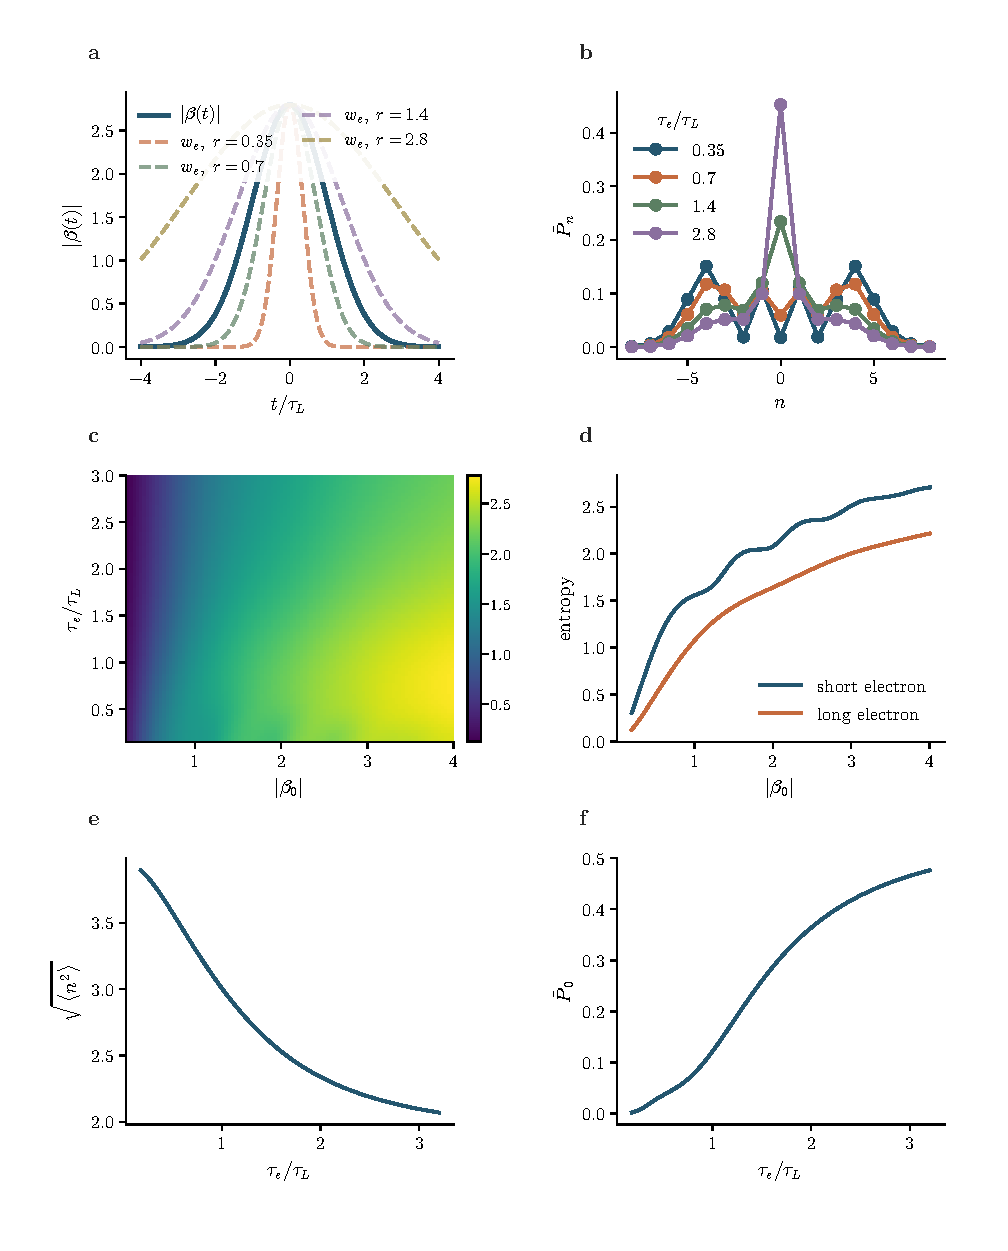
\includegraphics[width=0.96\linewidth,height=0.70\textheight,keepaspectratio]{finite_pulse.pdf}
\caption{\textbf{有限脉冲：时间重叠如何平均贝塞尔振荡}\quad 把瞬时耦合写成高斯包络，比较峰值耦合与时间积分后的实验能谱。}
\label{fig:ch01-story-extensions--09-finite-pulse}
\end{figure}

数值实现中，显式进行电子到达时间上的非相干平均，而非将峰值 $\beta_0$ 直接代入：
\[\beta(t)=\beta_0e^{-t^2/(2\tau_L^2)},\quad w_e(t)=\frac{e^{-t^2/(2\tau_e^2)}}{\int \dd t'\,e^{-t'^2/(2\tau_e^2)}},\quad\overline P_n=\int \dd t\,w_e(t)J_n^2(2|\beta(t)|),\quad S=-\sum_n\overline P_n\ln\overline P_n.\]
采用 $\beta_0=2.8$，无量纲 $t/\tau_L\in[-4,4]$（600 点）、$n=-8,\ldots,8$；$\tau_e/\tau_L=0.35,0.7,1.4,2.8$。熵图扫描 $|\beta_0|\in[0.2,4]$（100 点）与 $\tau_e/\tau_L\in[0.15,3]$（90 点）；新增图以 $[0.18,3.2]$ 的 64 个比值计算 $\overline P_0$ 和 $\sqrt{\sum_n n^2\overline P_n}$。有限边带截断按所得权重重新归一化。

具体到各面板，(a) 同时绘制光学包络 $\beta_0e^{-T^2/2}$ 和四个电子权重的\emph{峰值重标度} $\beta_0w_e(T)/\max w_e$；(b) 用 $T\in[-4,4]$ 的 600 点梯形积分，输出每个 $r=\tau_e/\tau_L$ 下的 $\bar P_n$（此图\emph{未}重新归一化到 $|n|\le8$ 内）；(c) 对 $r\in[0.15,3]$ 的 90 点与 $\beta_0\in[0.2,4]$ 的 100 点，先对截断概率归一，再取 $S=-\sum\bar P_n\ln\bar P_n$；(d) 在 (c) 中取最邻近 $r=0.35,2.8$ 的离散行；(e,f) 在 $r\in[0.18,3.2]$ 的 64 点、$\beta_0=2.8$ 上由同一截断归一分布计算 $\sqrt{\sum n^2\bar P_n}$ 与 $\bar P_0$。有限积分窗与不同子图的归一化规则是数值选择，不能遗漏。


\medskip
把前面得到的相位匹配、耦合强度和探测分辨率放在同一组坐标中，可以直接判断一个实验点最终会落在弱耦合、可分辨多边带还是反冲修正开始重要的区域。这里不再引入新模型，只比较已经定义的控制量。


从复耦合到实验图像之间还隔着两种平均：电子束横向尺寸使不同入射位置采样不同的近场，能量探测器又把离散边带与仪器响应卷积。为了说明这些过程如何同时改变“图像长什么样”和“图像含有多少可反演信息”，\cref{fig:ch01-nearfield-to-spectrum} 用同一个规定的高斯近场从头计算电场、轨迹耦合、边带谱和探测 Fisher 信息。图中局域电场是可控的解析代理，而不是对某个未知材料宣称完成了 Maxwell 自洽求解。

\begin{figure}[!htbp]
\centering
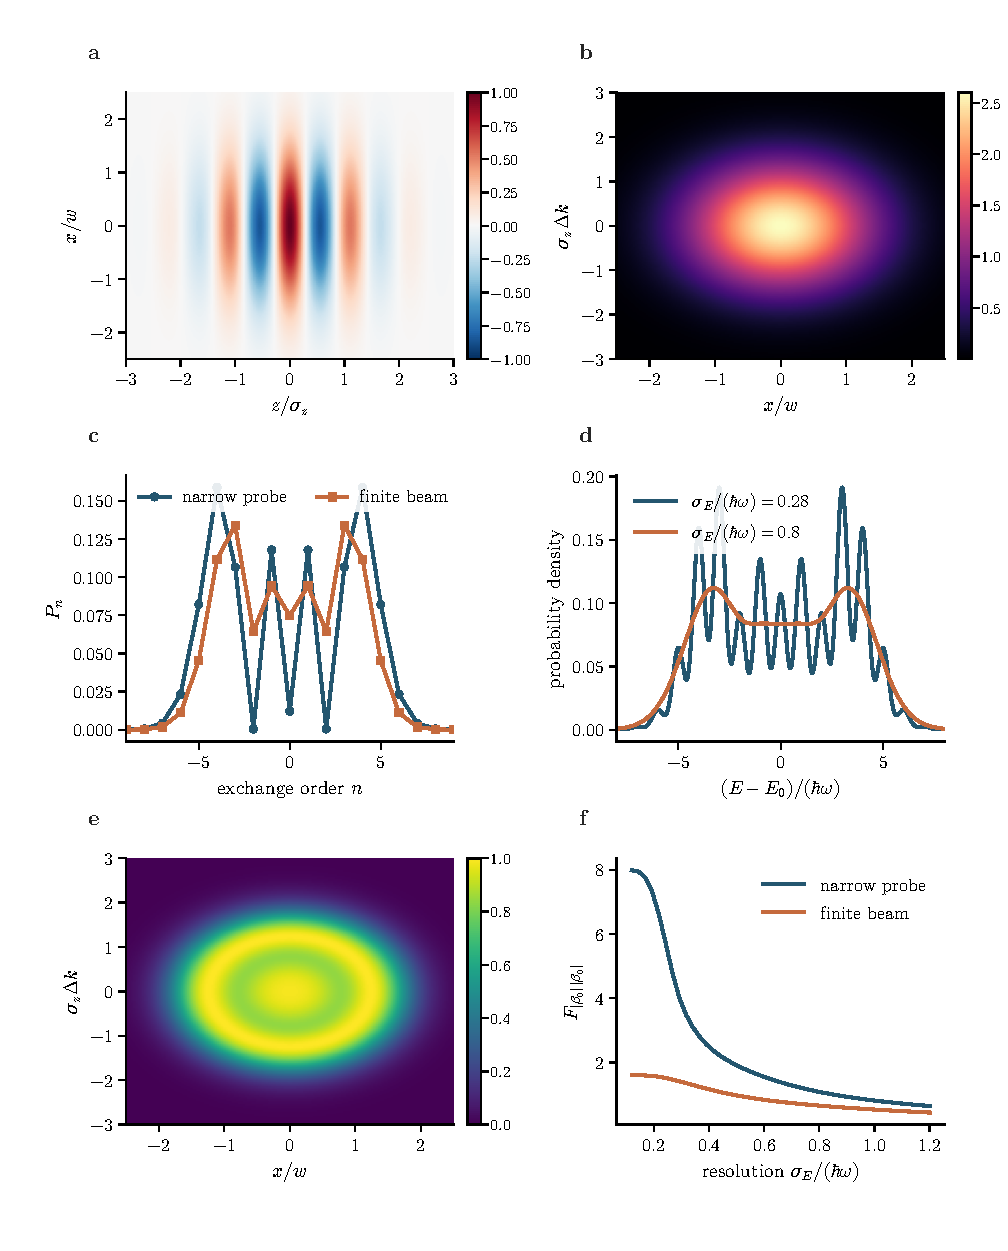
\includegraphics[width=0.97\linewidth,height=0.70\textheight,keepaspectratio]{nearfield_to_spectrum.pdf}
\caption{\textbf{从近场傅里叶分量到实验测量的完整链条。} (a) 规定纵向复电场的实部及其横向包络；(b) 沿电子轨迹做解析 Fourier 积分，得到关于束斑位置和纵向失配的复耦合幅值；(c) 将束腰中心的理想边带与横向非相干平均后的边带比较；(d) 进一步对同一边带人口做两种能量分辨率卷积；(e) 将场幅值转化为实际的非零边带信号 $1-P_0$，直观看出 PINEM 信号并不随场强单调变化；(f) 在固定前向模型下计算耦合幅度的经典 Fisher 信息，显示束斑平均和仪器展宽分别如何削弱反演精度。}
\label{fig:ch01-nearfield-to-spectrum}
\end{figure}

数值实现中，该图采用可解析、无量纲的规定近场（并非特定材料的 Maxwell 解）
\[
E_z(x,z)=E_0\exp\!\left[-\frac{x^2}{2w^2}-\frac{z^2}{2\sigma_z^2}\right]e^{\ii k_z z},
\qquad
\beta(x,\Delta k)=\beta_0\exp\!\left[-\frac{x^2}{2w^2}-\frac{(\sigma_z\Delta k)^2}{2}\right],
\]
其中 $\Delta k=k_z-\omega/v$，$\beta_0=eE_0\sqrt{2\pi}\sigma_z/(2\hbar\omega)=2.6$；所有长度以 $w,\sigma_z$ 无量纲化。(a) 在 $z/\sigma_z\in[-3,3]$ 的 301 点及 $x/w\in[-2.5,2.5]$ 的 261 点上绘 $\operatorname{Re}E_z/E_0$，专为可视化取 $k_z\sigma_z=5.5$；(b) 取 $\sigma_z\Delta k\in[-3,3]$ 的 181 点绘 $|\beta|$；(e) 在同一网格计算 $1-J_0^2(2|\beta|)$。(c) 的横向入射强度权重为 $W(x)\propto\exp[-x^2/(2\sigma_b^2)]$、$\sigma_b=0.65w$，按 $x$ 的 261 点梯形积分计算
\[
\overline P_n=\int W(x)J_n^2\!\left(2\beta_0e^{-x^2/(2w^2)}\right)\dd x,
\quad \int W(x)\dd x=1,
\]
并与束心 $P_n=J_n^2(2\beta_0)$ 比较；截断 $-13\le n\le13$ 后做离散归一。(d) 使用 $\hbar\omega=1$ 作能量单位及 $E/\hbar\omega\in[-10,10]$ 的 1001 点网格，以宽度 $\sigma_E/(\hbar\omega)=0.28,0.8$ 的归一化高斯核对同一 $\overline P_n$ 卷积，最后在有限画图区间做单位面积归一。(f) 令探测概率密度为卷积结果 $p(E;\beta_0)$，计算每电子经典信息
\[
F_{\beta_0\beta_0}=\int\frac{[\partial_{\beta_0}p(E;\beta_0)]^2}{p(E;\beta_0)}\,\dd E,
\]
导数使用 $\delta\beta_0=0.012$ 中心差分；连续扫描 $\sigma_E/(\hbar\omega)\in[0.12,1.2]$ 共 45 点，并分别对束心与横向平均后的分布求值。分母数值地板 $10^{-13}$ 仅防零除，不代表背景率。


\noindent \figref{fig:ch01-novel-extensions--33-recoil-approximation-breakdown}：六面板计算逐项核对。\par\noindent (a,b) 在 $K\in[1,300]$ keV 的 150 个对数点和光子能量 $0.5$--$5$ eV 的 150 点上，分别取 $n=1,50$ 画 $\log_{10}\max(\epsilon_q,10^{-14})$；(c) 固定 $\hbar\omega=2.4$ eV、$K=5,30,200$ keV，逐阶取 $1\le n\le100$；(d) 令 $n=1$ 对比 $q^{\rm ex}$ 和 $n\omega/v$；(e) 固定 $n=20$、$\hbar\omega=1,2.4,5$ eV，画 $\epsilon_q(K)$，虚线 $10^{-3}$ 只是选定精度判据；(f) 固定 $n=20$、$\hbar\omega=2.4$ eV，把 $\Delta q(K)L$ 作为相位失配，扫 $L=10\,\mathrm{nm}$--$10\,\mu\mathrm m$，阈值 $0.1$ rad 不是实验测得常数。


图 (b) 与 (e) 尤其值得对照：即使 $|\beta|$ 是规则的高斯包络，$J_0^2(2|\beta|)$ 的振荡也会把它映射成带有环状极值的 PINEM 响应。电子束平均后的边带仍具有明确的光子阶数，却不能再直接用“某一个束心处的 $\beta$”拟合全部人口；如果进一步丢失相邻边带的能量分辨率，参数辨识又会变差。这些效应都发生在经典 PINEM 框架内部，而不需要引入额外的量子退相干。
\clearpage


\par\medskip
实验能谱给出的是电子在各能量阶上的概率；相干态还保有各阶之间的相对相位。接着让电子离开近场并自由漂移，传播色散将这些相位转化为纵向密度调制，能谱成像与阿秒压缩便成为同一波函数演化的两个观察面。
\section{相空间传播}
PINEM 后的电子态写成


\begin{equation}
|\psi(0)\rangle=\sum_n c_n|E_0+n\hbar\omega\rangle.
\label{eq:ch02-1}
\end{equation}


系数 $c_n$ 是复数。$|c_n|^2$ 给出第 $n$ 阶边带人口，$\arg c_n$ 给出该分量的谱相位。能谱只能测到人口，而时间压缩依赖不同 $n$ 之间的相位差，所以还必须研究自由传播如何改变这些相位。

纵向波数为 $k(E)=p(E)/\hbar$。在 $n\hbar\omega\ll E_0$ 时，以 $E_0$ 为中心展开：


\begin{equation}
k(E_0+n\hbar\omega)=k_0+\frac{n\omega}{v}+\frac12\left.\frac{\dd ^2k}{\dd E^2}\right|_{E_0}(n\hbar\omega)^2+O(n^3).
\label{eq:ch02-2}
\end{equation}


在传播因子 $\ee^{\ii k(E)L}$ 中，$k_0L$ 只产生整体相位，$n\omega L/v$ 对应传播时间 $L/v$ 的平移。令迟滞时间 $t_r=t-L/v$，并在其对应的相位坐标 $\theta=\omega t_r$ 下讨论波包；保留到二次色散时，剩余传播相位可写成


\begin{equation}
c_n(L)=c_n(0)\ee^{-\ii\alpha n^2},\qquad \alpha=-\frac{L}{2}\left.\frac{\dd ^2k}{\dd E^2}\right|_{E_0}(\hbar\omega)^2.
\label{eq:ch02-3}
\end{equation}


这里已略去共同相位和线性相位，并将 $c_n(L)$ 理解为迟滞时间坐标中的系数。由相对论关系 $E^2=p^2c^2+m_e^2c^4$ 可得 $\dd ^2k/\dd E^2=-1/(\hbar\gamma^3m_ev^3)$，因此 $\alpha=L\hbar\omega^2/(2\gamma^3m_ev^3)>0$。这个无量纲参数控制各阶之间的二次相位差。

令 $\theta=\omega t_r$（下文如无特别说明，$t$ 表示相对于平均飞行时间的坐标），电子时间包络为


\begin{equation}
\psi(\theta;L)=\sum_n c_n(0)\ee^{-\ii n\theta}\ee^{-\ii\alpha n^2},\qquad I(\theta;L)=|\psi(\theta;L)|^2.
\label{eq:ch02-4}
\end{equation}


若许多边带在某个 $\alpha$ 处获得合适的相对相位，它们会在同一 $\theta$ 附近同相叠加，形成窄密度峰。由此可见，宽能谱只是压缩的必要条件；真正决定峰值位置和宽度的是谱相位。


\cref{eq:ch02-4} 中每个能量分量都有自己的振幅和相位。要形成窄时间峰，必须同时满足两个条件：边带范围足够宽，使波包具备较大的可用带宽；相位又必须在某个传播距离附近对齐，使这些分量能够同相叠加。只有宽能谱而没有正确相位，只会得到复杂振荡，不会自动得到阿秒压缩。

\begin{figure}[!htbp]
\centering
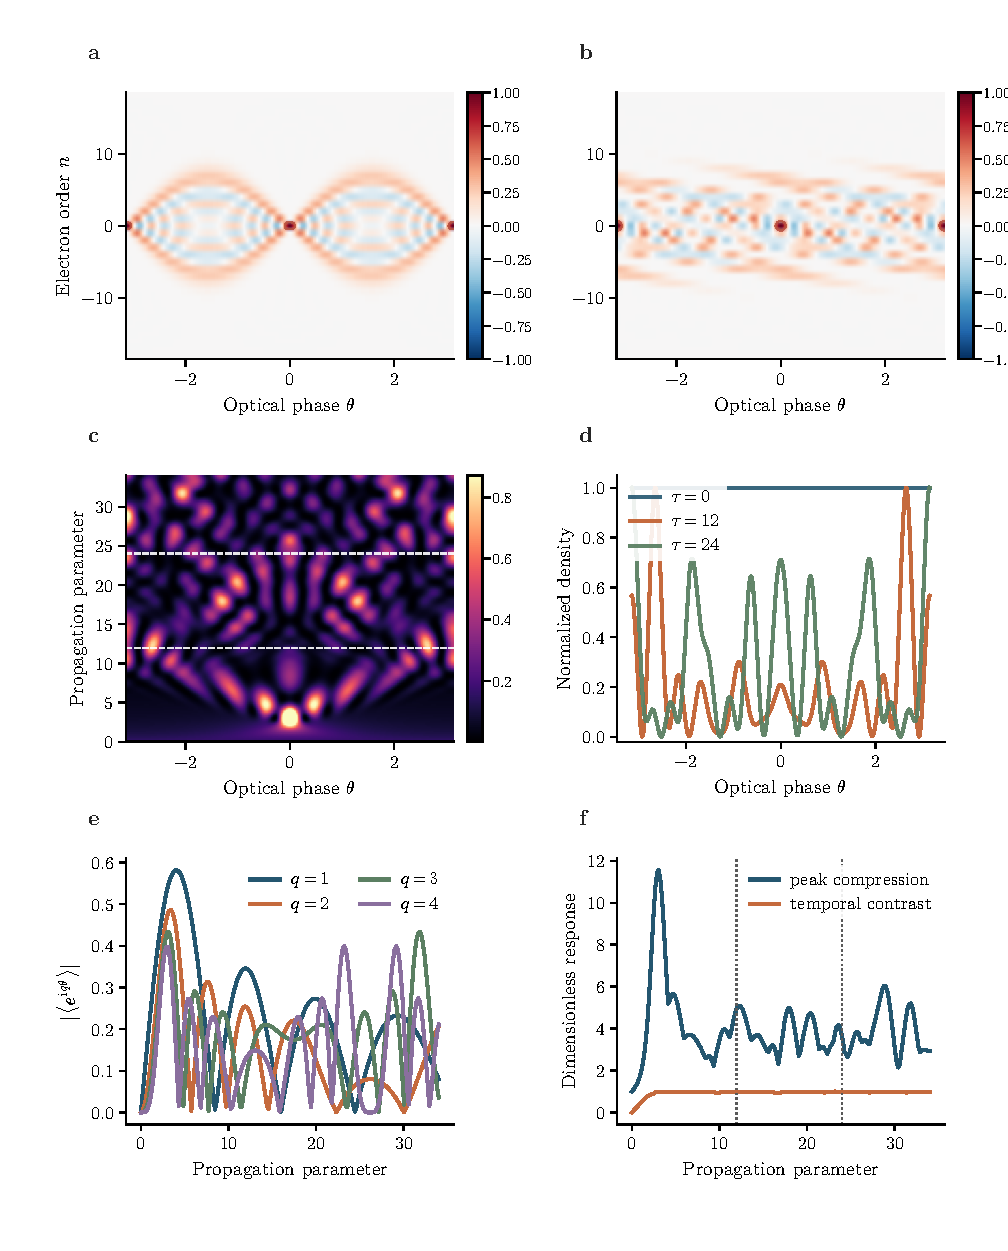
\includegraphics[width=0.96\linewidth,height=0.70\textheight,keepaspectratio]{feist2015_attosecond_phase_space.pdf}
\caption{\textbf{阿秒相空间整形}\quad PINEM 先建立离散能量梳，自由传播再给第 $n$ 阶分量积累与 $n^2$ 成正比的相位。上排直接画出周期 Wigner 相空间：初态的平滑能量--相位纹理在传播后被剪切并折叠，在最佳聚焦附近形成明显的焦散结构。右上角的传播图把这种剪切投影到时间轴，显示阿秒脉冲列如何在传播中生成与再聚焦。下排则把这一几何过程转成可读观测量：波形截面给出脉冲压缩与部分回波，谐波 bunching 因子显示不同空间频率何时被放大，而峰值压缩与时间对比度则把“好看”的波形转成可比较的定量指标。}
\label{fig:ch02-theory-atlas--08-feist2015-attosecond-phase-space}
\end{figure}

使用离散能量梳及其传播二次相位，纵向强度为
\[c_n(\tau)=i^nJ_n(2g)\ee^{-\ii D\tau n^2},\quad \psi(\theta,\tau)=\sum_{n=-n_c}^{n_c}c_n(\tau)\ee^{-\ii n\theta},\quad I(\theta,\tau)=\frac{|\psi|^2}{\int_{-\pi}^{\pi}|\psi|^2\dd \theta}.\]
取 $g=3.8$、$D=0.03$；周期 Wigner 图取 $n_c=18$ 与 320 个相位点，传播强度取 $n_c=22$、$\tau\in[0,34]$（190 点）、相位 440 点，而截面在 700 点相位网上重算 $\tau=0,12,24$。峰值压缩因子 $\max_\theta I(\theta,\tau)/\max_\theta I(\theta,0)$；新增对比度 $(I_{\max}-I_{\min})/(I_{\max}+I_{\min})$。这里 $D\tau$ 是无量纲传播参数，并未指定唯一的实验漂移长度。


当谱相位近似二次时，一个“最佳聚焦距离”通常就能概括主要动力学；多色调制或更高阶色散会让这种简单图像失效。此时 Wigner 分布更合适，因为它把局部频率（能量）和纵向位置同时展开。相空间中的折叠、剪切和多值映射在投影到时间轴时会形成焦散；高亮边界对应许多相空间轨迹在同一位置聚集，而不是新的相互作用通道。


时间密度 $I(t)=|\psi(t)|^2$ 只能告诉我们电子在什么时候出现，却不能唯一确定不同能量边带之间的相位。对一般混态，更基本的对象是能量基中的密度矩阵 $\rho_{nm}$。对角元 $\rho_{nn}$ 给出能谱人口，非对角元 $\rho_{nm}$ 则保存相干性；自由传播距离 $L$ 只是在这些矩阵元上积累已知相位，
\begin{equation}
\rho_{nm}(L)=\rho_{nm}(0)\exp\!\left[-\ii\alpha(n^2-m^2)\right]
\end{equation}
这里在迟滞时间坐标中保留二次传播相位；若谱宽较大，还须把 $k(E)$ 的三阶及更高阶项加入指数。该式表明对角人口 $\rho_{nn}$ 不变，而非对角元的相位随 $n^2-m^2$ 演化。于是“形成一个很窄的密度峰”和“制备了一个高纯度、相位已知的电子量子态”不是同一句话：前者只需要某一时刻的 $I(t)$ 很窄，后者要求足够多的 $\rho_{nm}$ 被实验约束。

Priebe 等在 2017 年的 SQUIRRELS 实验中已经把这个区别变成了实际层析问题：未知电子态先经过一个相位可控的参考光场，参考相互作用把不同 $\rho_{nm}$ 旋转到可测能量人口，再由多组参考相位的能谱反演密度矩阵。\textsuperscript{\hyperref[ch02-ref3]{[11]}} 这与普通 PINEM 拟合的根本差别在于，拟合 $P_n$ 只使用密度矩阵对角线，而量子态层析要利用受控幺正变换把非对角信息转到对角线。

2024 年的自由电子同频检测进一步把这一思想变成显式的相位读出。设样品给电子施加弱相位调制 $g=|g|\ee^{\ii\phi_g}$，随后参考平面施加已知调制 $g_{\rm ref}=|g_{\rm ref}|\ee^{\ii\phi_{\rm ref}}$。两次作用相干相加，弱信号极限下第一阶边带的对称组合含有
\begin{equation}
P_{+1}+P_{-1}\;\propto\; |g|\,|g_{\rm ref}|\cos(\phi_{\rm ref}-\phi_g)+\text{常数},
\label{eq:ch02-homodyne}
\end{equation}
因此扫描参考相位就能同时得到样品调制的幅度和相位。Gaida 等用这一方案在纳米尺度上重建了亚光周期近场演化。\textsuperscript{\hyperref[ch02-ref4]{[12]}} 这件事对后续研究很重要：很多“阿秒分辨”问题真正缺的不是更窄的电子密度峰，而是一个能把复响应的相位稳定地转成计数差的读出基。

这一结果还表明，单一参考相位只能测量某些复幅度组合。若未知样品响应同时含有多个谐波 $g_k$、幅度调制 $a_k$ 和部分相干性，那么单一参考相位扫描一般不再足够。可以把实验设计写成一个测量映射
\begin{equation}
\mu_j=\operatorname{Tr}\!\left[M_j(\boldsymbol\phi_{\rm ref})\rho_e\right],
\end{equation}
再问测量算符集合 $\{M_j\}$ 是否对目标密度矩阵或响应参数信息完备。测量反演章节的 Fisher 信息与贝叶斯反演正好可以接在这里：阿秒电子学的下一步不只是继续压缩脉冲，而是设计最少的参考设置来稳定恢复最多的相位信息。

当传播相位不仅用于形成脉冲，还要控制相干辐射的频率结构时，仍可沿用前面的同一套谱相位描述。区别只在于最终观察的是电子密度，还是由电子密度驱动的辐射场。\textsuperscript{\hyperref[ch02-ref5]{[13]}}
前面的讨论把二次谱相位当成电子自身的传播效应：它决定什么时候形成阿秒密度峰。2026 年 9 月 Zhu 等进一步指出，同一个二次相位还可以成为光源的可编程资源。电子先被制备成相干动量阶梯，再在漂移区获得确定的 $n^2$ 相位；这些相位一方面决定电子密度的 Talbot 谐波，另一方面可以在后续电子--光子作用与能量分辨电子读出中转移到光场，用于合成多分量薛定谔猫态。

密度谐波与传播相位的关系可从\cref{eq:ch02-4} 直接推导。把时间密度写成傅里叶级数
\begin{equation}
I(\theta;\alpha)=\sum_{q\in\ZZ}b_q(\alpha)\ee^{-\ii q\theta},
\label{eq:ch02-bunching-series}
\end{equation}
代入 $\psi(\theta;\alpha)=\sum_n c_ne^{-\ii n\theta-\ii\alpha n^2}$，第 $q$ 个密度谐波就是
\begin{equation}
b_q(\alpha)=\sum_n c_{n+q}c_n^*
\exp\!\left\{-\ii\alpha\left[(n+q)^2-n^2\right]\right\}.
\label{eq:ch02-bunching-factor}
\end{equation}
推导时把 $I=\psi\psi^*$ 展开为双重求和，并按指数 $\ee^{-\ii q\theta}$ 收集 $q=(n+q)-n$ 的交叉项；每一项对应相距 $q$ 个能量阶的两条相干路径。自由传播没有改变 $|c_n|^2$，却改变了这些路径在密度谐波中的相对相位。所谓 Talbot 选择，本质上就是选择一个 $\alpha$，使目标 $q$ 的求和尽量同相，而非目标谐波发生相消。

利用
\begin{equation}
(n+q)^2-n^2=2nq+q^2,
\end{equation}
可以看到相位随 $n$ 线性扫描，扫描斜率为 $2q\alpha$。当 $\alpha/\pi$ 取有理数时，这组相位在离散能量阶上周期复现，于是出现整数或分数 Talbot 结构。这个写法比“某个距离处出现窄脉冲”更强，因为它直接告诉我们怎样选择特定辐射谐波：优化目标不再只是最小化电子脉宽，而可以最大化 $|b_q|$ 并同时压低其他 $|b_{q'}|$。

Zhu 等的工作把这一步继续接到量子光。若后续光学模式与电子相互作用，电子的不同能量阶会携带已经编程好的二次相位进入联合散射；再对电子末态做能量分辨后选择，光场获得的条件振幅会继承这些路径相位。论文据此提出多分量猫态合成。这里最值得带走的不是某一张猫态 Wigner 图，而是一个新的设计原则：\emph{漂移区本身可以承担量子门的一部分}。原来需要在相互作用区通过复杂光场实现的相位操作，可以先由电子的确定性色散编译，再由后续散射把相位转给辐射场。

这也改变了阿秒电子学的优化目标。若最终任务是相干短波辐射，应优化 $b_q$；若任务是量子光条件制备，应优化条件态保真度、成功概率和对 $\alpha$ 噪声的鲁棒性；只有在“产生最窄电子密度峰”这一任务下，FWHM 才是自然目标。三个目标使用同一组 $c_n$ 和 $\alpha$，但最优点一般不会相同。

压缩宽度不能只靠增加 $|\beta|$ 无限减小。更宽的边带确实提供更大的频谱带宽，但也要求更多能量分量保持稳定的相对相位。初始能散、相位噪声、电子脉冲包络和高阶色散都会破坏这种相干，因此最终宽度由“可用带宽”和“可保持相干的带宽”中较小的一项决定。


纵向相空间控制有两条代表性的实验路线。Feist 等从光学相位调制出发，让自由传播把谱相位转成阿秒密度结构；Baum 则用太赫兹近场直接施加近似线性的能量啁啾，再用独立的时间偏转器测量压缩结果。

PINEM 路线中，Feist 等把相干能量梳的二次传播相位直接转成阿秒脉冲列。\textsuperscript{\hyperref[ch02-ref1]{[9]}}
在近场出口处，各能量边带已经相干叠加，但电子密度并不会立刻变成阿秒尖峰。论文把传播看成纵向相空间的剪切：不同动量分量具有不同群速度，因而原本主要写在相位里的调制逐渐转成时间密度调制。

论文图 3 给出的数值例子使用 $|g|=5.7$。在约 1.8 mm 的传播距离处，Wigner 分布被剪切到时间轴投影最窄的位置，形成周期为光学周期 $T=2.55$ fs、单峰约 82 as FWHM 的脉冲列。再继续传播，波包重新展宽并可出现复现。


另一条 THz 路线由 Baum 等实现：时间相关纵向力直接旋转相空间，并用第二个场把时间映射到可测偏转。\textsuperscript{\hyperref[ch02-ref2]{[10]}}
这篇工作与光学 PINEM 的离散边带不同，但它给出了非常清楚的纵向相空间控制实验。第一个近场谐振器工作在 THz 场零交叉附近：早到电子被减速，晚到电子被加速，于是时间—能量分布获得近似线性啁啾。自由漂移后，快慢电子在时间上会聚，形成时间焦点。

第二个 THz 谐振器不再负责压缩，而是把到达时间映射成横向偏转，因此它相当于条纹相机。实验把约 930 fs 的电子脉冲压到 75 fs FWHM，约为 12 倍压缩；同时报告了数飞秒量级的长期同步稳定性。

因此这篇论文的物理故事是“线性能量啁啾 → 漂移聚焦 → 独立时间偏转读出”，而不是把压缩和测量混成一个拟合参数。


设 PINEM 后只有 $n=-1,0,1$ 三个分量，并先取相同实振幅 $c_{-1}=c_0=c_1=1/\sqrt3$。自由传播只给第 $n$ 阶分量乘上 $\ee^{-\ii\alpha n^2}$，所以


\begin{equation*}
\psi(\theta)=\frac{1}{\sqrt3}\left(\ee^{\ii\theta-i\alpha}+1+\ee^{-\ii\theta-i\alpha}\right)
=\frac{1}{\sqrt3}\left[1+2\ee^{-\ii\alpha}\cos\theta\right].
\end{equation*}


于是强度为


\begin{equation*}
I(\theta)=\frac13\left(1+4\cos^2\theta+4\cos\alpha\cos\theta\right).
\end{equation*}


此例中三个边带的人口始终是 $1/3$，但 $\alpha$ 改变交叉项 $4\cos\alpha\cos\theta$，因而调节了时间密度的形状。当 $\cos\alpha$ 改变符号时，密度峰的位置也随之移动。真实 PINEM 态包含更多 $n$，但每一对边带的干涉仍由相对谱相位控制，因此后面的压缩图本质上是在寻找许多阶数能够同时相长干涉的 $\alpha$。


把 $|\beta|$ 与传播相位同时作为自变量，可以直接寻找时间峰最窄的区域。耦合增强会引入更多边带，有利于压缩；但参与干涉的分量越多，对相位误差越敏感。因此最佳工作区通常位于参数平面内部，而不是简单出现在最大耦合处。


改变初始啁啾、多色相对相位和传播距离，可以区分三种作用：谱振幅决定哪些能量分量参与干涉，二次谱相位决定主要聚焦位置，高阶谱相位决定波形是否发生折叠和焦散。Talbot 复现和焦散都可由同一组传播相位得到，不需要另外引入纵向力。

\begin{figure}[!htbp]
\centering
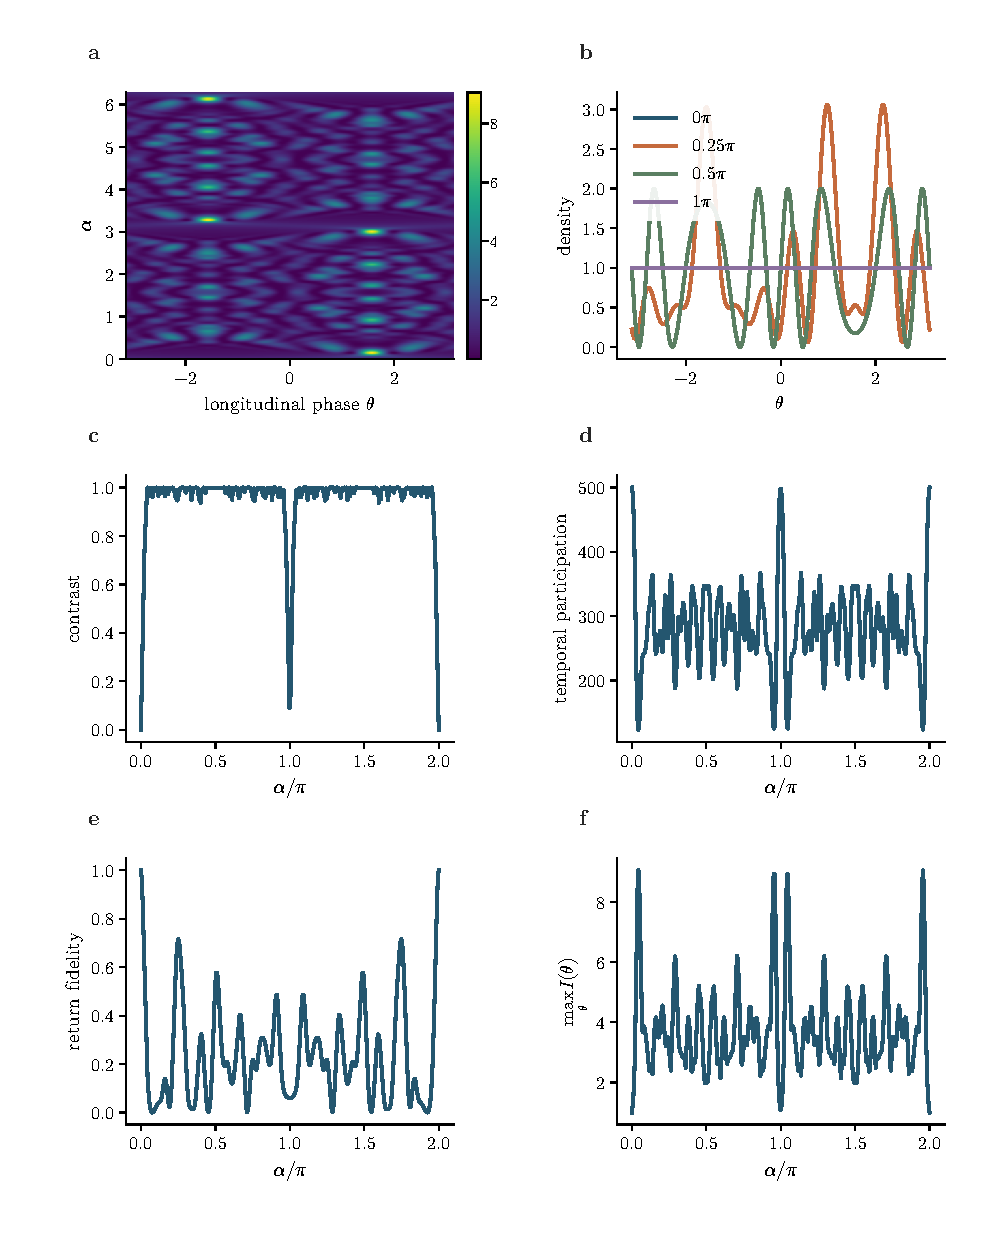
\includegraphics[width=0.96\linewidth,height=0.70\textheight,keepaspectratio]{talbot_revival.pdf}
\caption{\textbf{能量晶格中的 Talbot 复现}\quad 离散边带的二次谱相位会周期性重相干；这给出压缩之外的复现 / 分数复现图像。}
\label{fig:ch02-story-extensions--13-talbot-revival}
\end{figure}

计算周期谱相位的复现和返回保真度：
\[c_n=J_n(5.2),\quad I(\theta,\alpha)=\left|\sum_{n=-18}^{18}c_ne^{-i\alpha n^2+in\theta}\right|^2,\quad \mathcal F(\alpha)=\left|\sum_n|c_n|^2\ee^{-\ii\alpha n^2}\right|^2.\]
取 $\alpha\in[0,2\pi]$（360 点），$\theta\in[-\pi,\pi]$（500 点）；比较 $\alpha=0,\pi/4,\pi/2,\pi$。参与度由 $(\sum_\theta I)^2/\sum_\theta I^2$ 定义，其数值依赖 $\theta$ 采样点数；因此图中仅用于比较同一离散化下的相对变化。其余曲线为峰值密度、对比度和上述 $\mathcal F$。

具体到各面板，(a) 逐点输出 $I(\theta,\alpha)$，取 $|n|\le18$、$\theta$ 的 500 点及 $\alpha$ 的 360 点；(b) 画 $\alpha=0,\pi/4,\pi/2,\pi$ 的强度切片；(c) 画 $V=(I_{\max}-I_{\min})/(I_{\max}+I_{\min})$；(d) 画离散参与数 $N_{\rm eff}=(\sum_jI_j)^2/\sum_jI_j^2$，它随 500 点取样改变，不能解读为连续时间宽度；(e) 画严格的初态返回保真度 $\mathcal F=|\sum_n|c_n|^2\ee^{-\ii\alpha n^2}|^2$，$\alpha=\pi$ 的平移复现与 $\alpha=2\pi$ 的全态返回不同；(f) 在每个 $\alpha$ 求 $\max_\theta I$。全部曲线都来自同一离散复振幅，没有额外的任意复现包络。


\begin{figure}[!htbp]
\centering
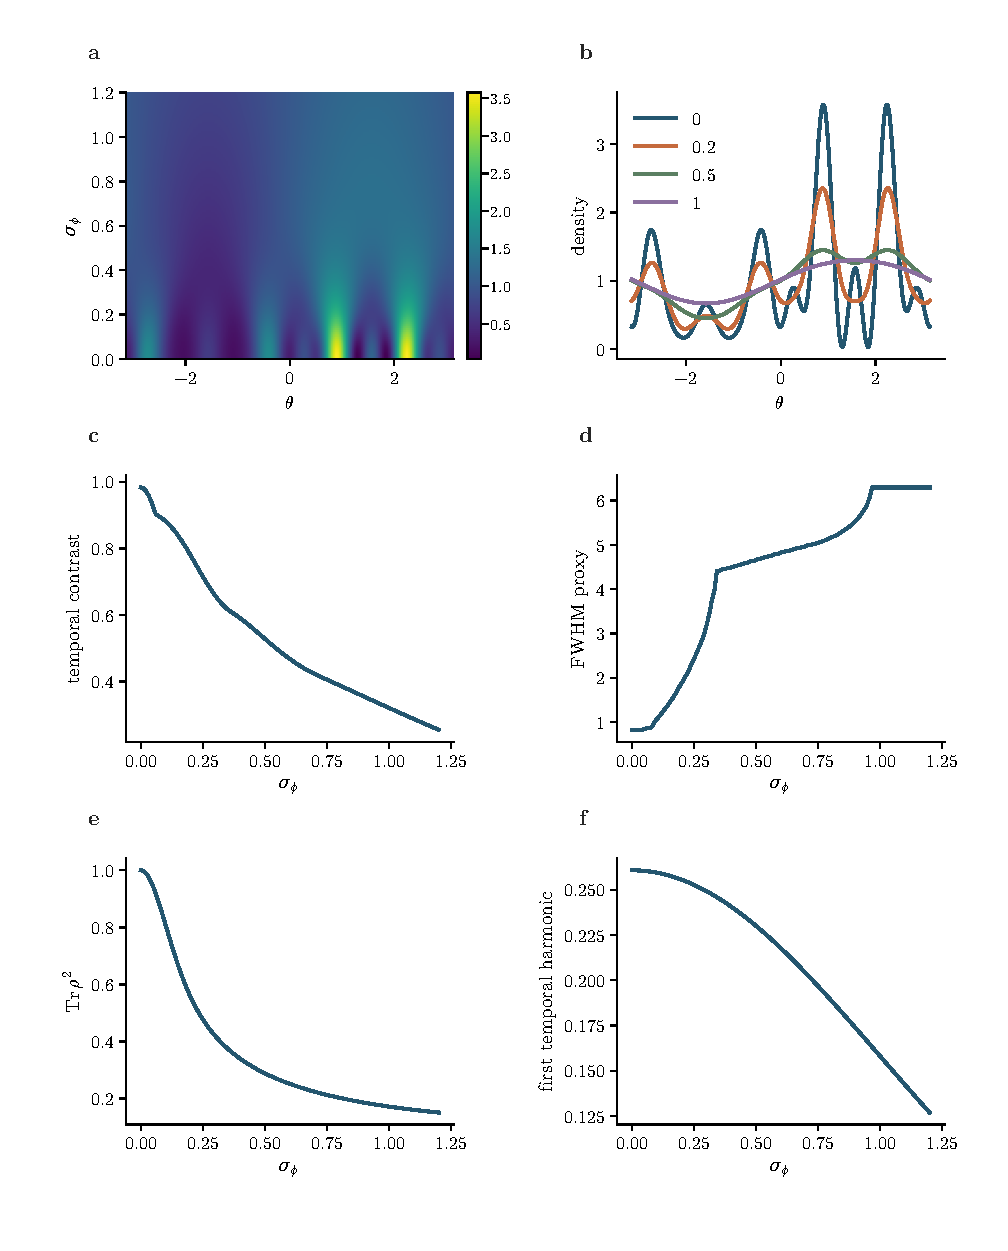
\includegraphics[width=0.96\linewidth,height=0.70\textheight,keepaspectratio]{phase_noise_attosecond.pdf}
\caption{\textbf{相位噪声对阿秒结构的破坏}\quad 同样的边带人口在相位扩散下可以完全失去时间压缩；因此能谱宽并不等价于阿秒脉冲短。}
\label{fig:ch02-story-extensions--17-phase-noise-attosecond}
\end{figure}

数值实现中，将高斯随机相位噪声写成密度矩阵退相干核：
\[\rho_{nm}=J_n(5)J_m(5)\ee^{-\ii0.48(n^2-m^2)}e^{-(n-m)^2\sigma_\phi^2/2},\quad I(\theta)=\sum_{n,m}\rho_{nm}\ee^{\ii(m-n)\theta},\quad \mathcal P=\sum_{nm}|\rho_{nm}|^2.\]
取 $n,m\in[-18,18]$，$\sigma_\phi\in[0,1.2]$（120 点），$\theta\in[-\pi,\pi]$（500 点）；截面 $\sigma_\phi=0,0.2,0.5,1$。除密度、对比度外，图中给出离散网格半高宽代理量、纯度 $\mathcal P$ 和一阶时间谐波 $|\int I(\theta)\ee^{\ii\theta}\dd \theta|/(2\pi)$。半高宽仅按网格阈值计数，不等于连续极限下严格的单峰 FWHM。


\noindent \figref{fig:ch02-theory-atlas--08-feist2015-attosecond-phase-space}：六面板计算逐项核对。\par\noindent
(a,b) 对同一离散电子能量梳在 $\tau=0$ 和 $\tau=12$ 计算周期 Wigner 准分布 $W(\theta,n)$，取 $|n|\le18$、$320$ 个相位采样点；这里使用等间隔能量格点的周期相空间表示，颜色可为负，不是经典联合概率。(c) 由 $c_n(\tau)=\ii^nJ_n(7.6)\ee^{-\ii(0.03)\tau n^2}$ 计算 $I(\theta,\tau)$，$\tau\in[0,34]$ 共 $190$ 点、$\theta$ 共 $440$ 点、$|n|\le22$；颜色上限为全部采样值的 $99.7$ 百分位，以免少数尖峰压暗其余纹理。(d) 分别在 $\tau=0,12,24$ 重算强度截面，每条曲线各除以自身峰值，因此这格只比较形状，不能直接比较绝对密度。(e) 对 (c) 的同一传播密度取 $q=1,2,3,4$ 阶聚束系数 $B_q(\tau)=|\int_{-\pi}^{\pi}I(\theta,\tau)\ee^{\ii q\theta}\dd\theta|$，数值积分采用 440 点梯形法；(f) 计算峰值压缩 $\max I(\tau)/\max I(0)$ 与 $V=(I_{\max}-I_{\min})/(I_{\max}+I_{\min})$。两条虚线仅标识参考传播参数 $\tau=12,24$，不表示已经满足某种严格的全态复现条件。

具体到各面板，(a) 对每个 $\sigma_\phi$ 由密度矩阵 $\rho_{nm}$ 计算 $I(\theta)$，$\theta$ 500 点、$\sigma_\phi$ 120 点；(b) 取最邻近 $\sigma_\phi=0,0.2,0.5,1$ 的采样行；(c) $V=(I_{\max}-I_{\min})/(I_{\max}+I_{\min})$；(d) 计算 $\Delta\theta\sum_j\mathbf1[I_j>I_{\max}/2]$，因可能有多个峰，这是半高阈值支持集长度，\emph{不是}严格 FWHM；(e) $\mathcal P=\sum_{n,m}|c_n|^2|c_m|^2e^{-(n-m)^2\sigma_\phi^2}$；(f) $|\int_{-\pi}^\pi I(\theta)\ee^{\ii\theta}\dd \theta|/(2\pi)$，用离散梯形积分。相位噪声是指定的高斯相干核，而不是由微观主方程推导的唯一环境。


\medskip
能量调制本身只决定谱系数；真正的时间结构还取决于自由传播积累的谱相位、初始啁啾和相位噪声。把这些量并列后，可以直接看出压缩位置为什么移动、复现为什么出现，以及相干性不足时哪些细结构最先消失。


\medskip
PINEM 首先在能量空间写入幅度与相位，自由传播再利用电子色散把谱相位转换为时间密度，因此“能量调制”和“阿秒压缩”是两个连续步骤。

二次谱相位 $\ee^{-\ii\alpha n^2}$ 是 Talbot 复现、分数复现和时间聚焦的共同数学来源；它还决定密度谐波的 bunching factor，因此 Zhu 等 2026 能把同一漂移相位用于选择相干辐射谐波并向条件量子光制备转移。

Feist 2015 证明了光学近场可以相干调制自由电子能量阶梯；Kealhofer 等 2016 则从 THz 相空间旋转与条纹读出展示了纵向相空间控制和计量的实验路径。

任何脉冲宽度下界都依赖实际带宽、相位噪声、高阶色散和探测响应；只用理想带宽给出的数值应理解为模型极限，而不是无条件实验分辨率。

能量与时间已经构成一个完整的纵向相空间描述。若相互作用还携带方位相位，电子态需要增加轨道角动量这一离散坐标，问题便从一维能量链扩展到合成维度。


双色光场不仅可以改变能量交换带宽，还能把相对光学相位变成控制时间焦散的旋钮。不过必须区分两步：PINEM 在作用区主要向电子写入的是\emph{时间相位}，没有后续色散时纯相位调制并不会立即产生阿秒强度峰；漂移区积累的 $n^2$ 谱相位才会把频谱干涉转换成时域密度压缩。\cref{fig:ch02-two-color-caustics} 以同一组贝塞尔卷积振幅计算了这整个过程。

\begin{figure}[!htbp]
\centering
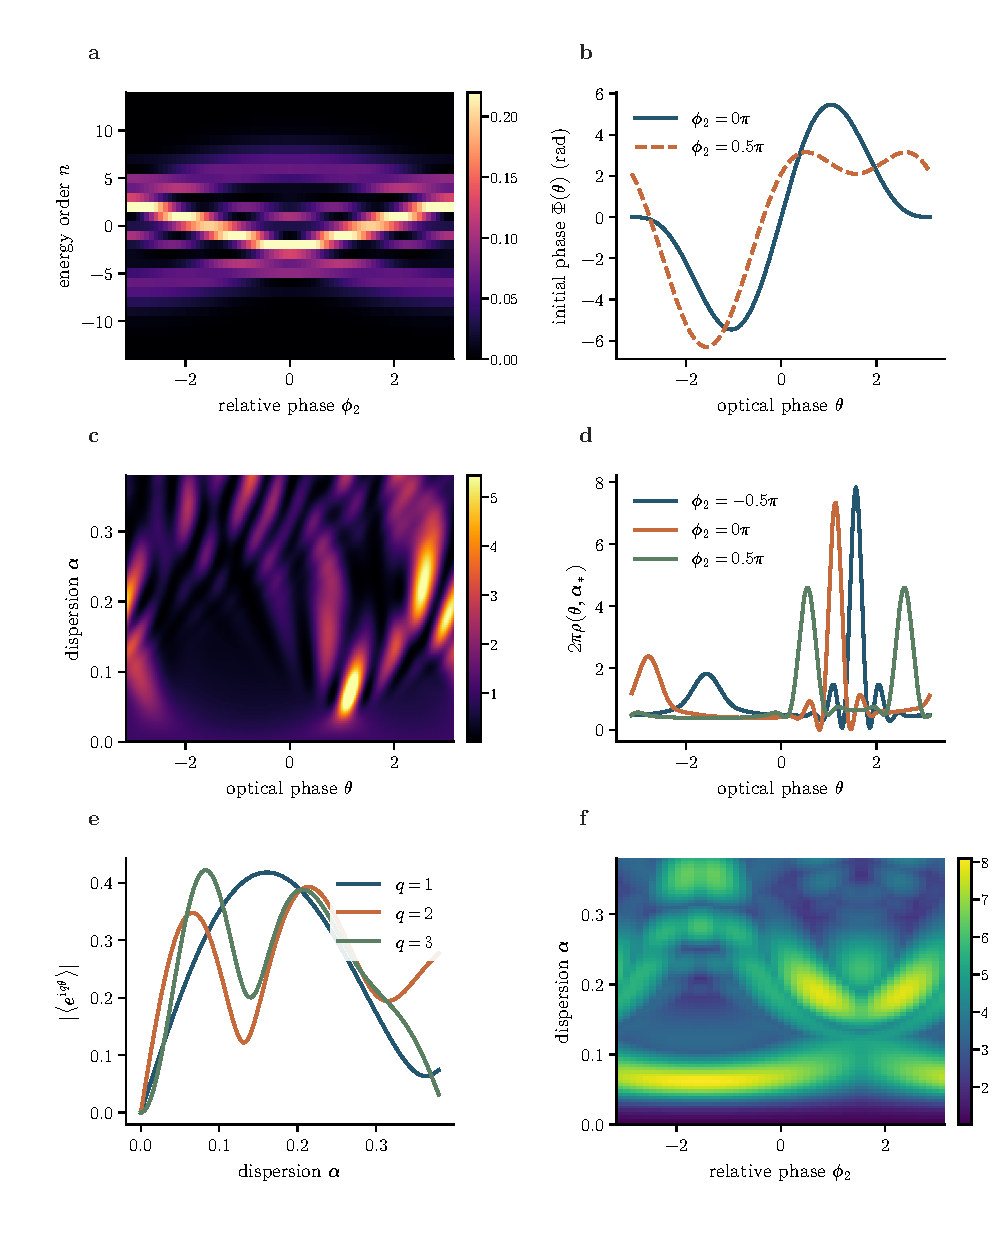
\includegraphics[width=0.97\linewidth,height=0.70\textheight,keepaspectratio]{two_color_temporal_caustics.pdf}
\caption{\textbf{双色驱动的能量路径干涉与阿秒焦散。} (a) 基频与二倍频散射路径相干叠加，边带人口随相对光学相位重新分配；(b) 作用区出口的两种光学相位函数，展示时间密度相同而相位调制不同的原因；(c) 传播二次谱相位使时间焦散逐渐形成；(d) 在同一传播距离处调节二倍频相位，改变脉冲峰形；(e) 第一到第三阶时间 bunching 因子量化各谐波结构的建立；(f) 在色散参数与相对相位平面扫描最强脉冲压缩，用同一前向模型寻找可优化的工作点。}
\label{fig:ch02-two-color-caustics}
\end{figure}

采用基频 $\omega$ 与二倍频 $2\omega$ 的理想相干调制，固定 $|\beta_1|=2.1$、$|\beta_2|=1.05$、$\phi_1=0$，相对光学相位记为 $\phi_2$。首先将落入相同能量阶数的所有两色路径相干相加：
\[
\widetilde c_n(\phi_2)=\sum_{n_1=-18}^{18}\sum_{n_2=-9}^{9}
J_{n_1}(2|\beta_1|)J_{n_2}(2|\beta_2|)
e^{\ii n_2\phi_2}\delta_{n,n_1+2n_2},\qquad
c_n=\frac{\widetilde c_n}{\sqrt{\sum_{m=-36}^{36}|\widetilde c_m|^2}}.
\]
把两个贝塞尔级数重新相乘，便能看出为何图 (b) 应比较调制相位而不是两条重合的强度曲线。对无限阶梯，Jacobi--Anger 恒等式直接给出
\begin{align*}
 \psi(\theta,0)&=\sum_{n\in\ZZ}c_n\ee^{\ii n\theta}\\
 &=\left[\sum_{n_1\in\ZZ}J_{n_1}(2|\beta_1|)\ee^{\ii n_1\theta}\right]
 \left[\sum_{n_2\in\ZZ}J_{n_2}(2|\beta_2|)\ee^{\ii n_2(2\theta+\phi_2)}\right]\\
 &=\exp\!\left\{\ii\left[2|\beta_1|\sin\theta+2|\beta_2|\sin(2\theta+\phi_2)\right]\right\}.
\end{align*}
因此传播前的模方恒等于 $1$，但相位函数随 $\phi_2$ 改变。有限截断 $c_n$ 近似这一精确恒等式，随后不同边带积累的二次相位才会把波函数的相位差转成可测时间密度差。

传播色散参数 $\alpha$ 使 $c_n\mapsto c_ne^{-\ii\alpha n^2}$。令 $\theta=\omega t$，取平均值为 1 的周期时间密度与 bunching 因子
\[
2\pi\rho(\theta,\alpha,\phi_2)=\left|\sum_{n=-36}^{36}c_n(\phi_2)e^{-\ii\alpha n^2}e^{\ii n\theta}\right|^2,
\qquad
B_q=\left|\frac{1}{2\pi}\int_{-\pi}^{\pi}2\pi\rho\,e^{\ii q\theta}\,\dd \theta\right|.
\]
(a) 使用 $\phi_2\in[-\pi,\pi]$ 的 71 点、$n=-36,\ldots,36$ 的通道绘 $|c_n|^2$，为避免过少强峰饱和，色标取第 $99.3$ 百分位；(b) 对 $\alpha=0$ 的纯相位调制，比较 $\phi_2=0,\pi/2$ 的解析相位 $\Phi(\theta)=2|\beta_1|\sin\theta+2|\beta_2|\sin(2\theta+\phi_2)$；两种情形的归一化强度均等于 $1$，故不再绘制重合的密度曲线；(c) 取 $\phi_2=0$、$\alpha\in[0,0.38]$ 共 114 点、$\theta\in[-\pi,\pi)$ 共 280 点，绘 $2\pi\rho$，色标截断在第 $99.5$ 百分位；(d) 在 (c) 最大峰密度对应的离散传播参数 $\alpha_*$ 处比较 $\phi_2=-\pi/2,0,\pi/2$；(e) 对 (c) 的同一分布计算 $B_1,B_2,B_3$；(f) 用 51 个 $\phi_2$ 与 83 个 $\alpha\in[0,0.38]$，逐点计算 $\max_\theta 2\pi\rho$。模型没有额外加入退相干、有限光脉冲、反冲与探测器响应。


双色驱动之外，三色相干光场还能进一步调节时间射线映射的高阶驻相结构。这里不把“出现尖锐峰”直接称作一种新奇点，而先给出可检验的驻相判据。设无损、忽略反冲的相位调制为
\begin{equation}
 f(\theta_0)=\exp\!\left[\ii\Phi(\theta_0)\right],\qquad
 \Phi(\theta_0)=2\sum_{j=1}^{3}|\beta_j|\sin(j\theta_0+\varphi_j),
 \qquad c_n=\frac1{2\pi}\int_{-\pi}^{\pi} f(\theta_0)\ee^{-\ii n\theta_0}\,\dd \theta_0 .
 \label{eq:ch02-three-color-phase}
\end{equation}
经过无量纲二次谱色散 $\tau$ 后，电子波形严格由
\begin{equation}
 \psi(\theta,\tau)=\sum_{n=-n_{\max}}^{n_{\max}}c_n \ee^{\ii n\theta-\ii\tau n^2}
 \label{eq:ch02-three-color-wave}
\end{equation}
给出，数值上应检查 $n_{\max}$ 收敛。只有当参与的边带足够多、可以对离散和采用驻相近似时，才引入辅助的“射线”变量 $\theta_0$：条件 $n=\Phi'(\theta_0)$ 与传播群延迟共同给出
\begin{equation}
 \theta=\theta_0+2\tau\Phi'(\theta_0),\qquad
 \frac{\partial\theta}{\partial\theta_0}=1+2\tau\Phi^{(2)}(\theta_0).
 \label{eq:ch02-caustic-ray}
\end{equation}
当雅可比因子为零时出现折叠焦散的经典投影；若同一点还满足 $\Phi^{(3)}(\theta_0)=0$，且进一步的高阶导数非零，才可能出现尖点型退化。Airy 和 Pearcey 函数分别描述这些退化驻相积分的局域一致近似，而不是有限边带和式的普适精确解。加入三色场主要增加了调整 $\Phi^{(2)}$、$\Phi^{(3)}$ 的独立旋钮，但色散高阶项、能谱截断和相位噪声都可能使理想尖点变钝。由此可以将“漂亮的焦散形状”转化为明确的实验问题：在相同的总边带带宽与噪声预算下，第三种颜色能否稳定增加可分辨的时间 bunching，而不只是移动一个峰的位置？

对照图 (a) 和 (b) 可见，边带人口分布发生变化，并不意味着电子在近场出口已形成时间峰。只有把图 (a) 的复振幅继续演化到图 (c)--(f)，才能判断哪一种相位设置真的改善压缩。多色相位控制因此同时具有谱学可观测量和漂移后的时域动力学后果。

\clearpage
\par\medskip 从近场耦合章节的 $\beta$ 到本章的飞行整形，只增加了一项物理：离开近场后各能量分量有不同的纵向动量。$n$ 的线性相位等价于波形平移，二次相位才会改变脉冲形状；因此把相位零点、群延迟与色散参数混为一个拟合量，就会误判聚焦位置。Talbot 图中 $\alpha=\pi$ 对应 $\ee^{-\ii\pi n^2}=(-1)^n$，是波形沿光学相位平移 $\pi$，而非原始态保真度必然回到一；真正的全态返回出现在 $\alpha=2\pi$。


\par\bigskip
\noindent{\small\textit{参考文献}\par\vspace{2pt}
\begin{enumerate}
\item \phantomsection\label{ch01-ref1}Barwick, B.; Flannigan, D. J.; Zewail, A. H. Photon-induced near-field electron microscopy. \emph{Nature} 462, 902--906 (2009). \href{https://doi.org/10.1038/nature08662}{\nolinkurl{doi:10.1038/nature08662}}.
\item \phantomsection\label{ch01-ref2}García de Abajo, F. J.; Asenjo-Garcia, A.; Kociak, M. Multiphoton Absorption and Emission by Interaction of Swift Electrons with Evanescent Light Fields. \emph{Nano Letters} 10, 1859--1863 (2010). \href{https://doi.org/10.1021/nl100613s}{\nolinkurl{doi:10.1021/nl100613s}}.
\item \phantomsection\label{ch01-ref3}Park, S. T.; Lin, M.; Zewail, A. H. Photon-induced near-field electron microscopy (PINEM): theoretical and experimental. \emph{New Journal of Physics} 12, 123028 (2010). \href{https://doi.org/10.1088/1367-2630/12/12/123028}{\nolinkurl{doi:10.1088/1367-2630/12/12/123028}}.
\item \phantomsection\label{ch01-ref4}Park, S. T.; Zewail, A. H. Relativistic Effects in Photon-Induced Near Field Electron Microscopy. \emph{J. Phys. Chem. A} 116, 11128--11133 (2012), with Supporting Information. \href{https://doi.org/10.1021/jp304534n}{\nolinkurl{doi:10.1021/jp304534n}}.
\item \phantomsection\label{ch01-ref5}Feist, A. et al. Quantum coherent optical phase modulation in an ultrafast transmission electron microscope. \emph{Nature} 521, 200--203 (2015). \href{https://doi.org/10.1038/nature14463}{\nolinkurl{doi:10.1038/nature14463}}.
\item \phantomsection\label{ch01-ref6}Rivera, N.; Kaminer, I. Light--matter interactions with photonic quasiparticles. \emph{Nature Reviews Physics} 2, 538--561 (2020). \href{https://doi.org/10.1038/s42254-020-0224-2}{\nolinkurl{doi:10.1038/s42254-020-0224-2}}.
\item \phantomsection\label{ch01-ref7}Li, J.; Zhao, L.; Liu, Y. Quantum optics with free electrons. \emph{Reviews of Modern Physics}, accepted 30 September 2026. \href{https://doi.org/10.1103/zy5t-r4lp}{\nolinkurl{doi:10.1103/zy5t-r4lp}}. 本书用其理论层级作为 2026 年领域坐标，而不把综述本身当作单一模型。
\item \phantomsection\label{ch01-ref8}Carlsen, M. B.; Madsen, L. B. Modulation of electron wave packets by scattering on time-harmonic potentials. \emph{Physical Review A} 114, 033117 (2026). \href{https://doi.org/10.1103/r76m-4zsk}{\nolinkurl{doi:10.1103/r76m-4zsk}}.
\item \phantomsection\label{ch02-ref1}Feist, A. et al. Quantum coherent optical phase modulation in an ultrafast transmission electron microscope. \emph{Nature} 521, 200--203 (2015). \href{https://doi.org/10.1038/nature14463}{\nolinkurl{doi:10.1038/nature14463}}.
\item \phantomsection\label{ch02-ref2}Kealhofer, C.; Schneider, W.; Ehberger, D.; Ryabov, A.; Krausz, F.; Baum, P. All-optical control and metrology of electron pulses. \emph{Science} 352, 429--433 (2016). \href{https://doi.org/10.1126/science.aae0003}{\nolinkurl{doi:10.1126/science.aae0003}}.
\item \phantomsection\label{ch02-ref3}Priebe, K. E. et al. Attosecond electron pulse trains and quantum state reconstruction in ultrafast transmission electron microscopy. \emph{Nature Photonics} 11, 793--797 (2017). \href{https://doi.org/10.1038/s41566-017-0045-8}{\nolinkurl{doi:10.1038/s41566-017-0045-8}}.
\item \phantomsection\label{ch02-ref4}Gaida, J. H. et al. Attosecond electron microscopy by free-electron homodyne detection. \emph{Nature Photonics} 18, 509--515 (2024). \href{https://doi.org/10.1038/s41566-024-01380-8}{\nolinkurl{doi:10.1038/s41566-024-01380-8}}.
\item \phantomsection\label{ch02-ref5}Zhu, S.; Zeng, Y.; Pan, C.; Pan, Y.; Tian, Y.; Li, R. Programming Coherent and Quantum Light with a Free-Electron Wavepacket. \emph{Physical Review Letters} 137, 143601 (2026). \href{https://doi.org/10.1103/k2cg-484h}{\nolinkurl{doi:10.1103/k2cg-484h}}.
\end{enumerate}
}
